\hypertarget{criterion2}{%
\chapter{Criterion 2: Program Learning Outcomes (PLOs)}\label{criterion2}}

% Keep all Criterion 2 figures within the printable page area while
% preserving their original aspect ratios and any specified widths.
\let\CriterionTwoOriginalIncludeGraphics\includegraphics
\renewcommand{\includegraphics}[2][]{%
  \CriterionTwoOriginalIncludeGraphics[height=0.72\textheight,keepaspectratio,#1]{#2}%
}

PLOs define the knowledge, skills, and professional attributes that students are expected to achieve by graduation, in accordance with the graduate attributes prescribed in the PEC Manual of Accreditation 2019. The BE Software Engineering program at NUST-SEECS has adopted these attributes as PLOs, with twelve PLOs for intake 2K23 and previous batches and a revised framework of eleven PLOs for intake 2K24 onwards. The PLOs are mapped to the PEOs, CLOs, and curriculum, and are assessed through direct methods, including coursework and Final Year Design Projects (FYDP), and indirect methods, including internship feedback and Graduate Exit Surveys. Individual student attainment is monitored against the minimum 50\% threshold, while cohort performance is evaluated against defined KPIs. Assessment results are reviewed by the department to identify gaps, implement corrective actions, and support continuous quality improvement of the program.

%-----------------------------------------------------------------------
\hypertarget{sec:3.1plos}{%
\section{PLOs: Software Engineering Program at SEECS}\label{sec:3.1plos}}

\hypertarget{sec:plosseecs}{%
\subsection{PLOs Applicable to the 2023 Intake and Earlier Batches}\label{sec:plosseecs}}

For students admitted to the BE Software Engineering program at SEECS in the 2023 intake and earlier, the program defines 12 PLOs, also referred to as Graduate Attributes (GAs). The 12 PLOs are listed below:

\begin{enumerate}
\item \textbf{PLO-1 Engineering Knowledge:} An ability to apply knowledge of mathematics, science, engineering fundamentals and an engineering specialization to the solution of complex engineering problems.
\item \textbf{PLO-2 Problem Analysis:} An ability to identify, formulate, research literature, and analyze complex engineering problems reaching substantiated conclusions using first principles of mathematics, natural sciences and engineering sciences.
\item \textbf{PLO-3 Design/Development of Solutions:} An ability to design solutions for complex engineering problems and design systems, components or processes that meet specified needs with appropriate consideration for public health and safety, cultural, societal, and environmental considerations.
\item \textbf{PLO-4 Investigation:} An ability to investigate complex engineering problems in a methodical way including literature survey, design and conduct of experiments, analysis and interpretation of experimental data, and synthesis of information to derive valid conclusions.
\item \textbf{PLO-5 Tool Usage:} An ability to create, select and apply appropriate techniques, resources, and modern engineering and IT tools, including prediction and modeling, to complex engineering activities, with an understanding of the limitations.
\item \textbf{PLO-6 The Engineer and Society:} An ability to apply reasoning informed by contextual knowledge to assess societal, health, safety, legal and cultural issues and the consequent responsibilities relevant to professional engineering practice and solution to complex engineering problems.
\item \textbf{PLO-7 Environment and Sustainability:} An ability to understand the impact of professional engineering solutions in societal and environmental contexts and demonstrate knowledge of and need for sustainable development.
\item \textbf{PLO-8 Ethics:} Apply ethical principles and commit to professional ethics and responsibilities and norms of engineering practice.
\item \textbf{PLO-9 Individual and Collaborative Team Work:} An ability to work effectively, as an individual or in a team, on multifaceted and /or multidisciplinary settings.
\item \textbf{PLO-10 Communication:} An ability to communicate effectively, orally as well as in writing, on complex engineering activities with the engineering community and with society at large, such as being able to comprehend and write effective reports and design documentation, make effective presentations, and give and receive clear instructions.
\item \textbf{PLO-11 Project Management:} An ability to demonstrate management skills and apply engineering principles to one's own work, as a member and/or leader in a team, to manage projects in a multidisciplinary environment.
\item \textbf{PLO-12 Lifelong Learning:} An ability to recognize importance of and pursue lifelong learning in the broader context of innovation and technological developments.
\end{enumerate}

\subsection{PLOs Applicable to the 2024 Intake and Onwards Batches}
\label{sec:plosseecs}

To align the Software Engineering curriculum with the revised Graduate Attributes framework of the International Engineering Alliance (IEA), which consolidates the attributes relating to society and environmental sustainability into a single outcome, the department revised its PLO framework from 12 to 11 outcomes for students admitted from Fall 2024 onwards\footnote{WP No. 20, 69th ACM}. The revised PLOs are listed below:

\begin{enumerate}
\item \textbf{PLO-1 Engineering Knowledge:} Apply knowledge of mathematics, natural science, engineering fundamentals and engineering specialization to the solution of complex engineering problems.
\item \textbf{PLO-2 Problem Analysis:} Identify, formulate, conduct research literature, and analyze complex engineering problems reaching substantiated conclusions using first principles of mathematics, natural sciences and engineering sciences.
\item \textbf{PLO-3 Design/Development of Solutions:} An ability to design solutions for complex engineering problems and design systems, components or processes that meet specified needs with appropriate consideration for public health and safety, cultural, societal, and environmental considerations.
\item \textbf{PLO-4 Investigation:} Conduct investigation of complex engineering problems using research-based knowledge and research methods, including design of experiments, analysis and interpretation of data, and synthesis of information to provide valid conclusions.
\item \textbf{PLO-5 Tool Usage:} Create, select and apply appropriate techniques, resources, and modern engineering and IT tools, including prediction and modeling, to complex engineering problems, with an understanding of the limitations.
\item \textbf{PLO-6 The Engineer and the World:} Analyze and evaluate sustainable development impacts to society, the economy, sustainability, health and safety, legal frameworks, and the environment while solving complex engineering problems.
\item \textbf{PLO-7 Ethics:} Apply ethical principles and commit to professional ethics and norms of engineering practice and adhere to relevant national and international laws. Demonstrate an understanding of the need for diversity and inclusion.
\item \textbf{PLO-8 Individual and Collaborative Team Work:} Function effectively as an individual, and as a member or leader in diverse and inclusive teams and in multi-disciplinary, face-to-face, remote and distributed settings.
\item \textbf{PLO-9 Communication:} Communicate effectively and inclusively on complex engineering activities with the engineering community and with society at large, such as being able to comprehend and write effective reports and design documentation, and make effective presentations, taking into account cultural, language, and learning differences.
\item \textbf{PLO-10 Project Management and Finance:} Demonstrate knowledge and understanding of engineering management principles and economic decision-making and apply these to one's own work, as a member and leader in a team, to manage projects in multidisciplinary environments.
\item \textbf{PLO-11 Lifelong Learning:} Recognize the need for, and have the preparation and ability for (i) independent and life-long learning (ii) adaptability to new and emerging technologies and (iii) critical thinking in the broadest context of technological change.
\end{enumerate}

The PLOs applicable to the respective batches are publicized and available on the SEECS website\footnote{https://seecs.nust.edu.pk/department-page/obe-peo-plo/}, SEECS notice boards, posters in corridors, and on LMS.

%-----------------------------------------------------------------------
\hypertarget{sec:plopeo}{%
\section{Mapping of PLOs to PEOs}\label{sec:plopeo}}

The aforementioned PLOs collectively contribute to achieving the PEOs. The relationship between the PLOs and PEOs is illustrated through the mappings provided in Table~\ref{table3.1} and Table~\ref{table3.2}, with the corresponding rationale detailed in Annexure~\ref{app:criteria-2_plo-peo_mapping_rationale}.

\begin{table}[hb]
\footnotesize
\centering
\caption{PLOs to PEOs Mapping (Intake 2K23 and Previous Batches) \textit{PEO-1: Demonstrate sound software engineering knowledge and skill set}; \textit{PEO-2: Lead diverse teams and work collaboratively to develop innovative solutions}; \textit{PEO-3: Conduct professional practice for sustainable development with due consideration for societal, ethical and environmental aspects.}}
\begin{tabular}{>{\centering\arraybackslash}p{0.08\textwidth}
                >{\raggedright\arraybackslash}p{0.45\textwidth}
                >{\centering\arraybackslash}p{0.11\textwidth}
                >{\centering\arraybackslash}p{0.11\textwidth}
                >{\centering\arraybackslash}p{0.11\textwidth}}
\toprule
\textbf{S No} & \textbf{PLOs} & \textbf{PEO-1} & \textbf{PEO-2} & \textbf{PEO-3} \\
\midrule
1  & Engineering Knowledge              & $\checkmark$ & & \\
2  & Problem Analysis                   & $\checkmark$ & & \\
3  & Design/Development of Solutions    & $\checkmark$ & $\checkmark$ & \\
4  & Investigation                      & $\checkmark$ & & \\
5  & Modern Tool Usage                  & $\checkmark$ & & \\
6  & The Engineer and Society           & & & $\checkmark$ \\
7  & Environment and Sustainability     & & & $\checkmark$ \\
8  & Ethics                             & & & $\checkmark$ \\
9  & Individual and Teamwork            & & $\checkmark$ & \\
10 & Communication                      & & $\checkmark$ & \\
11 & Project Management                 & & $\checkmark$ & \\
12 & Lifelong Learning                  & $\checkmark$ & & \\
\bottomrule
\end{tabular}
\label{table3.1}
\end{table}

\begin{table}
\footnotesize
\centering
\caption{PLOs to PEOs Mapping (Intake 2K24 and Onward Batches) \textit{PEO-1: Demonstrate sound software engineering knowledge and skill set}; \textit{PEO-2: Lead diverse teams and work collaboratively to develop innovative solutions}; \textit{PEO-3: Conduct professional practice for sustainable development with due consideration for societal, ethical and environmental aspects.}}
\begin{tabular}{>{\centering\arraybackslash}p{0.08\textwidth}
                >{\raggedright\arraybackslash}p{0.45\textwidth}
                >{\centering\arraybackslash}p{0.11\textwidth}
                >{\centering\arraybackslash}p{0.11\textwidth}
                >{\centering\arraybackslash}p{0.11\textwidth}}
\toprule
\textbf{S No} & \textbf{PLOs} & \textbf{PEO-1} & \textbf{PEO-2} & \textbf{PEO-3} \\
\midrule
1  & Engineering Knowledge                  & $\checkmark$ & & \\
2  & Problem Analysis                       & $\checkmark$ & & \\
3  & Design/Development of Solutions        & $\checkmark$ & $\checkmark$ & \\
4  & Investigation                          & $\checkmark$ & & \\
5  & Tool Usage                             & $\checkmark$ & & \\
6  & The Engineer and the World             & & & $\checkmark$ \\
7  & Ethics                                 & & & $\checkmark$ \\
8  & Individual and Collaborative Team Work & & $\checkmark$ & \\
9  & Communication                          & & $\checkmark$ & \\
10 & Project Management and Finance         & & $\checkmark$ & \\
11 & Lifelong Learning                      & $\checkmark$ & & \\
\bottomrule
\end{tabular}
\label{table3.2}
\end{table}

%\textbf{Mapping Summary}
%\begin{itemize}
%\item PEO-1 (Technical Competence): Supported by PLOs 1, 2, 3, 4, 5, and 11.
%\item PEO-2 (Leadership and Collaboration): Supported by PLOs 3, 8, 9, and 10.
%\item PEO-3 (Professional and Sustainable Practice): Supported by PLOs 6 and 7.
%\end{itemize}


%-----------------------------------------------------------------------
\hypertarget{sec:ploga}{%
\section{Encompassment of Graduate Attributes through PLOs}\label{sec:ploga}}

As mentioned in previous section, the program follows a framework of 12 PLOs for students admitted in the 2023 intake and earlier and a revised framework of 11 PLOs for students admitted from the 2024 intake onwards. Both frameworks are designed to encompass the applicable Graduate Attributes (GAs) and ensure that graduates develop the required knowledge, skills, and professional competencies. The comprehensive coverage of these attributes is demonstrated through systematic mapping of PLOs to GAs, with corresponding course mapping establishing how each PLO is addressed and progressively developed across the curriculum. The alignment of PLOs with CLOs, curriculum content, and teaching and learning activities supports the progressive development of the competencies associated with each GA. CLOs are formulated at appropriate levels of Bloom's Taxonomy, while direct and indirect assessment mechanisms provide evidence of students' attainment of the intended outcomes. Direct assessment includes quizzes, assignments, laboratory work, projects, presentations, and examinations, while indirect evidence is obtained through structured Internship Feedback and the Graduate Exit Survey.

PLO assessment results are reviewed through the CQI process to identify gaps in attribute coverage or attainment and to inform improvements in curriculum content, teaching and learning strategies, assessment methods, and outcome mapping. Separate mappings for the 12-PLO and 11-PLO frameworks demonstrate the coverage of the applicable GAs for the respective intake cohorts. In the revised framework, the consolidation of the attributes relating to the engineer's role in society and environmental sustainability is reflected in the corresponding PLO mapping. This systematic alignment of GA with PLOs, courses, CLOs, and assessment mechanisms supports their comprehensive coverage and progressive development throughout the program.
%-----------------------------------------------------------------------
\hypertarget{sec:ploreview}{%
\section{Review Process of PLOs \& Involvement of Stakeholders}\label{sec:ploreview}}

PLO attainment is evaluated through both direct and indirect assessment methods. Direct assessment is conducted through the curriculum at the individual student and cohort (batch) levels, while indirect assessment is carried out through internship feedback and exit surveys. Individual-level assessment monitors the attainment of PLOs by each student, whereas cohort-level assessment helps identify deficiencies and areas for improvement at the program level. Indirect assessment provides additional stakeholder-based evidence for evaluating program effectiveness and supporting CQI. Assessment data is collected and reviewed at the end of each academic semester, while overall PLO attainment at the program level is evaluated at the graduation of each batch. The assessment results are reviewed by the LQEC, which initiates corrective or improvement actions where required. These actions may progressively be taken up by the relevant responsible bodies, including the FBS, in accordance with the hierarchy shown in Figure~\ref{fig:plo-cqi-process}. The key stakeholders involved in the PLO assessment and CQI process include faculty, students, and industry. Faculty contributes through course delivery and direct assessment, students through exit surveys, and industry through feedback on student performance during internships. The flow chart in Figure~\ref{fig:plo-cqi-process} summarizes the overall PLO assessment, review, and CQI process.

\begin{figure}[H]
\centering
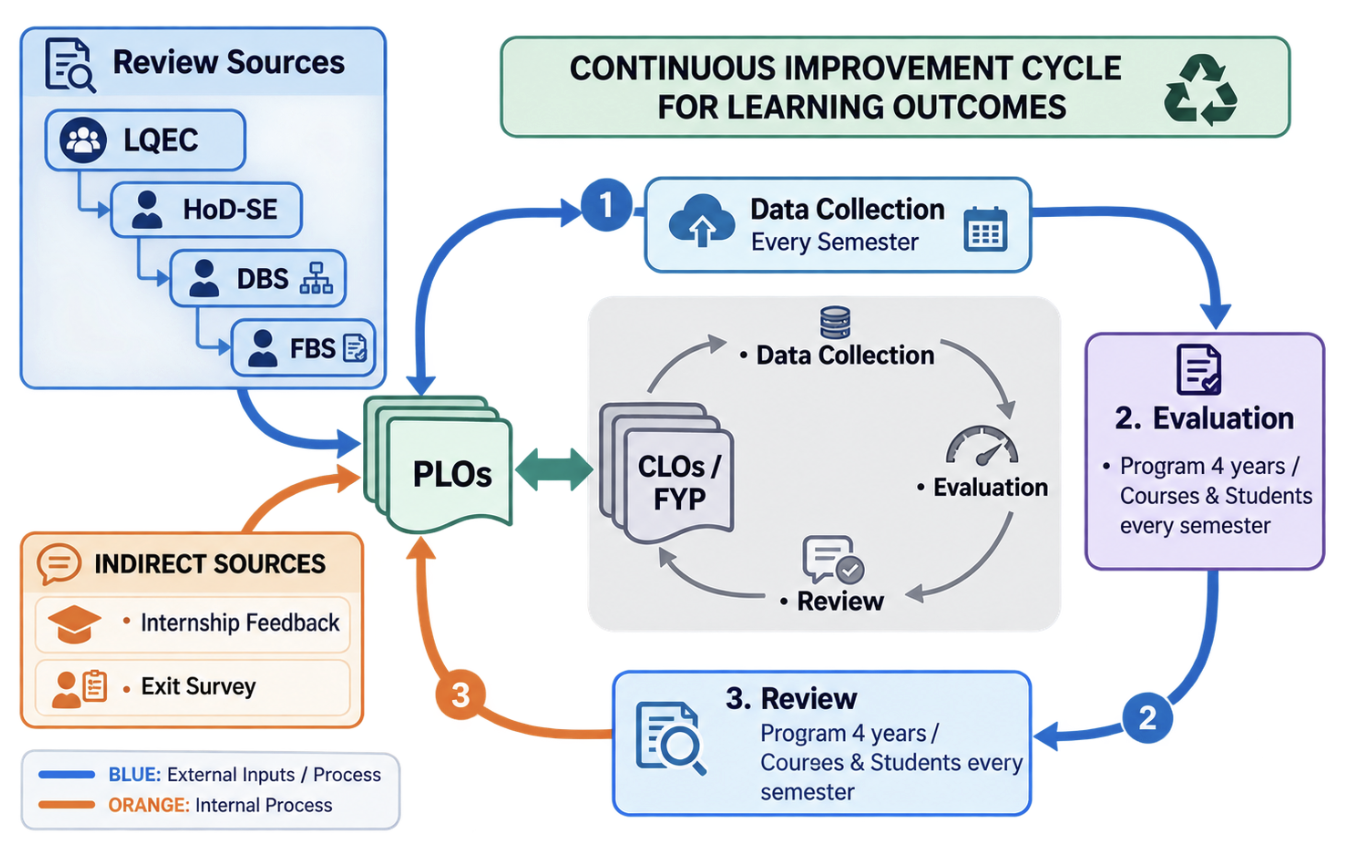
\includegraphics[width=0.80\textwidth]{images/front_matter/media/image-15.png}
\caption{PLO Assessment, Review, Stakeholder Involvement, and CQI}
\label{fig:plo-cqi-process}
\end{figure}

%-----------------------------------------------------------------------
\hypertarget{sec:cloplo}{%
\section{Mapping of Courses to PLOs}\label{sec:cloplo}}

To ensure comprehensive coverage of all 11 Program Learning Outcomes (PLOs), courses are systematically designed and mapped to relevant PLOs through their Course Learning Outcomes (CLOs). Rather than mapping every course to all PLOs, the curriculum adopts a structured, progressive approach in which selected courses contribute to the attainment of specific graduate attributes throughout the program.

The mapping of selected courses used for PLO assessment is presented in Table~\ref{table:courses-to-plo-mapping}. It demonstrates how individual CLOs contribute to relevant PLOs and how graduate attributes are developed across the curriculum. In addition to coursework, relevant PLOs are mapped to the Final Year Design Project (FYDP) evaluation rubrics used in Semesters 7 and 8. These rubrics assess students' attainment of the applicable graduate attributes at different stages of project development, providing evidence of their ability to apply engineering knowledge, solve complex problems, work collaboratively, and demonstrate professional competencies, as relevant to the mapped PLOs.

CLO achievement provides direct evidence of student learning and is systematically reviewed through the Continuous Quality Improvement (CQI) process. Assessment results help identify performance gaps, evaluate teaching and assessment strategies, and determine corrective actions where required. Similarly, FYDP rubric results contribute to evaluating PLO attainment through students' project planning, design, implementation, and final evaluation.

Course outlines are prepared by the concerned faculty in consultation with the Local Quality Enhancement Cell (LQEC) to ensure alignment with program objectives, relevant PLOs, and institutional quality assurance requirements. These outlines are reviewed and approved by the Head of Department (HoD). Subsequent revisions arising from course assessment, stakeholder feedback, or CQI recommendations are incorporated through the established review and approval process. A sample course outline is provided in Annexure~\ref{app:criteria-3_Course Outline with Knowledge Group Head's Signature}. Table~\ref{table:elective mapping} presents the mapping of CLOs of all specialization courses to PLOs, with equal weightage assigned to each contributing course outcome.

% Table 3.3: Course-to-PLO Mapping (wide table -- landscape + scriptsize)
\clearpage
\begin{landscape}
\begingroup\scriptsize\setlength{\tabcolsep}{2.5pt}
\begin{longtable}{>{\raggedright\arraybackslash}p{0.075\linewidth}
                  >{\raggedright\arraybackslash}p{0.165\linewidth}
                  >{\centering\arraybackslash}p{0.055\linewidth}
                  >{\centering\arraybackslash}p{0.055\linewidth}
                  >{\centering\arraybackslash}p{0.055\linewidth}
                  >{\centering\arraybackslash}p{0.055\linewidth}
                  >{\centering\arraybackslash}p{0.055\linewidth}
                  >{\centering\arraybackslash}p{0.055\linewidth}
                  >{\centering\arraybackslash}p{0.055\linewidth}
                  >{\centering\arraybackslash}p{0.055\linewidth}
                  >{\centering\arraybackslash}p{0.055\linewidth}
                  >{\centering\arraybackslash}p{0.055\linewidth}
                  >{\centering\arraybackslash}p{0.055\linewidth}
                  >{\centering\arraybackslash}p{0.065\linewidth}}
\caption{Mapping of Courses to PLOs and Appropriate BT Domain \& BT Level} \\
\toprule
\textbf{Code} & \textbf{Course Title} & \textbf{PLO 1} & \textbf{PLO 2} & \textbf{PLO 3} & \textbf{PLO 4} & \textbf{PLO 5} & \textbf{PLO 6} & \textbf{PLO 7} & \textbf{PLO 8} & \textbf{PLO 9} & \textbf{PLO 10} & \textbf{PLO 11} & \textbf{WKs} \\
& & \scriptsize Eng. Know. & \scriptsize Prob. Anal. & \scriptsize Design/ Dev. & \scriptsize Invest. & \scriptsize Tool Usage & \scriptsize Eng. \& World & \scriptsize Ethics & \scriptsize Teamwork & \scriptsize Commun. & \scriptsize Proj. Mgmt. & \scriptsize Lifelong Learn. & \\
\midrule
\endfirsthead
\multicolumn{14}{l}{\footnotesize\textit{Continued from previous page}} \\
\toprule
\textbf{Code} & \textbf{Course Title} & \textbf{PLO 1} & \textbf{PLO 2} & \textbf{PLO 3} & \textbf{PLO 4} & \textbf{PLO 5} & \textbf{PLO 6} & \textbf{PLO 7} & \textbf{PLO 8} & \textbf{PLO 9} & \textbf{PLO 10} & \textbf{PLO 11} & \textbf{WKs} \\
\midrule
\endhead
\midrule\multicolumn{14}{r}{\footnotesize\textit{Continued on next page}} \\
\endfoot
\bottomrule
\endlastfoot
\multicolumn{14}{l}{\textbf{Semester 1}} \\
CS-117   & Applications of ICT                       & C-2 & C-4 &     &     &     &     &     & A-3 &     &     &     & WK-2 \\
HU-131   & Fehm-ul-Quran I                           &     &     &     &     &     &     &     &     &     &     & C-2 & WK-7 \\
HU-101   & Islamic Studies                           &     &     &     &     &     & C-4 & A-3 &     &     &     & C-2 & WK-7 \\
CS-110   & Fundamentals of Computer Programming      & C-2 & C-3 &     &     & P-3 &     &     & A-2 &     &     &     & WK-2 \\
MATH-101 & Calculus and Analytical Geometry          & C-2, C-3 & C-4 &   &   &   &   &   &   &   &   &   & WK-2 \\
PH-102   & Applied Physics                           &     & C-3, C-3 & P-3 & & &  &  &  &  &  &  & WK-2 \\
HU-127   & Ideology and Constitution of Pakistan     &     &     &     &     &     & A-2 &     &     &     &     & C-4 & WK-7 \\
\multicolumn{14}{l}{\textbf{Semester 2}} \\
CS-212   & Object Oriented Programming               & C-2 & C-5 & C-6 &     & P-3 &     & A-3 &     &     &     &     & WK-3 \\
HU-132   & Fehm-e-Quran-II                           &     &     &     &     &     &     &     &     &     &     & C-2 & WK-7 \\
MATH-121 & Linear Algebra and ODEs                   & C-2 & C-3 & C-3 &     &     &     &     &     &     &     &     & WK-2 \\
MATH-161 & Discrete Mathematics                      & C-2 & C-4 & C-3 &     &     &     &     &     &     &     &     & WK-2 \\
HU-114   & Functional English                        &     &     &     &     &     &     &     &     & A-2 &     & C-2, C-3 & WK-7 \\
EE-122   & Computer Architecture and Logic Design    & C-3 & C-4 & C-5 & P-4 &  P-4   &     & A-3 & A-3 &     &     &     & WK-3 \\
\multicolumn{14}{l}{\textbf{Semester 3}} \\
CS-220   & Database Systems                          & C-2 &     & C-3 & C-5 & P-3 &     &     &     &     &     &     & WK-3 \\
SE-200   & Software Engineering                      & C-2 & C-4 & C-3 & C-5 &     &     &     & A-3 &     &     &     & WK-4 \\
CS-250   & Data Structures \& Algorithms             & C-2 &     & C-3   &  & P-4 &     & A-3 & A-2 &     &     &     & WK-3 \\
MATH-232 & Complex Variables and Transform           & C-3 & C-4 & C-5 &     &     &     &     &     &     &     &     & WK-2 \\
EE-353   & Computer Networks                         & C-3 &     & C-6 & C-4 & P-4 &     &     &     &     &     &     & WK-3 \\
\multicolumn{14}{l}{\textbf{Semester 4}} \\
CS-330   & Operating Systems                         & C-2 & C-4 &     & C-5 & P-3 &     &     &     &     &     &     & WK-3 \\
CS-251   & Design \& Analysis of Algorithm           &     & C-4 & C-6 & C-5 &     &     &     &     &     &     &     & WK-4 \\
HU-107   & Pakistan Studies                          &     &     &     &     &     &  & A-2 &     &     &     & C-2 & WK-7 \\
SE-211   & Software Design and Architecture          & C-2 & C-4 & C-3 & C-5 &     &     &     &     &     &     &     & WK-4 \\
MATH-361 & Probability and Statistics                & C-2 & C-4 & C-3 &     &     &     &     &     &     &     &     & WK-2 \\
ENGL-104 & Expository Writing                        &     &     &     &     &     & C-4 & C-3 &     & A-4    &     &  & WK-7 \\
\multicolumn{14}{l}{\textbf{Semester 5}} \\
MGT-121  & Introduction to Management                &     & C-4 &     &     &     &     &     &     & A-2 & A-3 & C-2 & WK-7 \\
CS-344   & Web Engineering*                          & C-2 & C-3 &     & C-4 & P-4 &     &     & A-2 &     &     &     & WK-5 \\
SE-315   & Cloud Computing                           & C-2 & C-3 &     & C-4 & P-4 &     &     &     &     &     &     & WK-4 \\
CS-336   & Embedded Systems                          & C-2, C-3 &  &  & P-4 & P-4 &  &  &  &  &  &  & WK-4 \\
HU-222   & Professional Ethics                       &     &     &     &     &     & C-4 & C-3 &     &     &     & A-3 & WK-7 \\
SE-314   & Software Construction                     & C-2 & C-3 & C-6 &     & P-3 &     &     &     &     &     &     & WK-4 \\
\multicolumn{14}{l}{\textbf{Semester 6}} \\
MGT-271  & Entrepreneurship                          &     &  C-4   &  C-3   &     &     & C-2  &  &  & A-3 & C-6 &  & WK-7 \\
SE-320   & Formal Methods                            & C-2 &     & C-6 & C-4 & P-3 &     &     &     &     &     &     & WK-3 \\
CS-471   & Machine Learning*                         & C-3 & C-4 & C-6 &     & P-4 &     &     &     &     &     &     & WK-5 \\
CS-261   & Human Computer Interaction                & C-2 & C-4 & C-6 &     & P-3 &     &     &     &     &     &     & WK-4 \\
SE-430   & Software Project Management               & C-2 &     &     & C-4 & C-5 &     &     & A-5 &     & A-3 &     & WK-4 \\
SE-321   & Software Quality Engg.                    & C-3 & C-4 & C-6 &     &     & A-3 &     &     &     &     &     & WK-4 \\
\multicolumn{14}{l}{\textbf{Semester 7}} \\
SE-498   & Final Year Design Project -- 1            & $\checkmark$ & $\checkmark$ & $\checkmark$ & $\checkmark$ & $\checkmark$ & $\checkmark$ &  & $\checkmark$ & $\checkmark$ & $\checkmark$ & & WK-6/7/8 \\
CS-484   & Information Security                      & C-2 &     & C-6 & C-4 &     &     &     &     &     &     &     & WK-4 \\
CS-365   & Virtual \& Augmented Reality*             & C-2 & C-4 & C-6 &     & P-4 &     &     &     &     &     &     & WK-6 \\
MATH-352 & Numerical Methods                         & C-3 & C-4 &  &     & P-4 &     &     &     &     &     &     & WK-2 \\
CS-335   & Internet of Things*                       & C-2 & C-4 & C-6 & C-5 &     &     &     &     &     &     &     & WK-4 \\
CS-381   & Network Security*                         & C-3 &     & C-6 & C-5 & P-3 &     &     &     &     &     &     & WK-5 \\
\multicolumn{14}{l}{\textbf{Semester 8}} \\
SE-499   & Final Year Design Project -- 2            & $\checkmark$ & $\checkmark$ & $\checkmark$ & $\checkmark$ & $\checkmark$ & $\checkmark$ & $\checkmark$ & $\checkmark$ & $\checkmark$ & $\checkmark$ & $\checkmark$ & WK-6/7/8 \\
ECO-130  & Engineering Economics*                    & C-2 & C-4 &     &     &     &     &     &     &     & C-5 &     & WK-7 \\
CS-416   & Large Language Models*                    & C-2 & C-4 & C-3 & C-5 & P-4 &     &     & C-6 &     &     &     & WK-6 \\
CCE-401  & Civic \& Community Engagement             &     &     &     &     &     & A-3, A-4 &     &     &     &    &     & WK-7 \\
OHS-101  & Occupation Health \& Safety               &     &     &     &     &     & C-3, C-2 &  &  &  &  &  & WK-3 \\
CS-415   & Mobile Application Development*           & C-2 &     & C-6 & C-4 & P-4 &     &     &     &     &     &     & WK-6 \\
\midrule
         & \textbf{Total}                            & \textbf{36} & \textbf{30} & \textbf{27} & \textbf{19} & \textbf{22} & \textbf{12} & \textbf{8} & \textbf{10} & \textbf{6} & \textbf{6} & \textbf{10} & \\
\label{table:courses-to-plo-mapping}
\end{longtable}

\vspace{12pt}
\textbf{*Elective Depth Courses}

\begin{longtable}{>{\raggedright\arraybackslash}p{0.075\linewidth}
                  >{\raggedright\arraybackslash}p{0.165\linewidth}
                  >{\centering\arraybackslash}p{0.055\linewidth}
                  >{\centering\arraybackslash}p{0.055\linewidth}
                  >{\centering\arraybackslash}p{0.055\linewidth}
                  >{\centering\arraybackslash}p{0.055\linewidth}
                  >{\centering\arraybackslash}p{0.055\linewidth}
                  >{\centering\arraybackslash}p{0.055\linewidth}
                  >{\centering\arraybackslash}p{0.055\linewidth}
                  >{\centering\arraybackslash}p{0.055\linewidth}
                  >{\centering\arraybackslash}p{0.055\linewidth}
                  >{\centering\arraybackslash}p{0.055\linewidth}
                  >{\centering\arraybackslash}p{0.055\linewidth}
                  >{\centering\arraybackslash}p{0.065\linewidth}}
\caption{Elective Depth Courses -- PLO Mapping} 
\label{table:elective mapping}
\\
\toprule
\textbf{Code} & \textbf{Course Title} & \textbf{PLO 1} & \textbf{PLO 2} & \textbf{PLO 3} & \textbf{PLO 4} & \textbf{PLO 5} & \textbf{PLO 6} & \textbf{PLO 7} & \textbf{PLO 8} & \textbf{PLO 9} & \textbf{PLO 10} & \textbf{PLO 11} & \textbf{WKs} \\
\midrule
\endfirsthead
\multicolumn{14}{l}{\footnotesize\textit{Continued from previous page}} \\
\toprule
\textbf{Code} & \textbf{Course Title} & \textbf{PLO 1} & \textbf{PLO 2} & \textbf{PLO 3} & \textbf{PLO 4} & \textbf{PLO 5} & \textbf{PLO 6} & \textbf{PLO 7} & \textbf{PLO 8} & \textbf{PLO 9} & \textbf{PLO 10} & \textbf{PLO 11} & \textbf{WKs} \\
\midrule
\endhead
\midrule\multicolumn{14}{r}{\footnotesize\textit{Continued on next page}} \\
\endfoot
\bottomrule
\endlastfoot
EC-303  & Mobile Application Development for SMEs & C-2 &     & C-6 & C-4 & P-4 &  &  &  &  &  &  & WK-6 \\
CS-335  & Internet of Things     & C-2 & C-4 & C-6 & C-5 &     &  &  &  &  &  &  & WK-4 \\
CS-344  & Web Engineering        & C-2 & C-3 &     & C-4 & P-4 &  &  & A-2 &  &  &  & WK-5 \\
CS-365  & Virtual and Augmented Reality & C-2 & C-4 & C-6 &  & P-4 &  &  &  &  &  &  & WK-6 \\
CS-368  & Reinforcement Learning & C-3 & C-4 & C-6 &     & P-3 &  &  &  &  &  &  & WK-6 \\
CS-381  & Network Security       & C-3 &     & C-6 & C-5 & P-3 &  &  &  &  &  &  & WK-5 \\
CS-405  & Deep Learning          & C-3 & C-4 & C-6 &     & P-4 &  &  &  &  &  &  & WK-6 \\
CS-416  & Large Language Models  & C-2 & C-4 & C-3 & C-5 & P-4 &  &  & C-6 &  &  &  & WK-6 \\
CS-471  & Machine Learning       & C-3 & C-4 & C-6 &     & P-4 &  &  &  &  &  &  & WK-5 \\
CS-481  & Computer Forensics     & C-2 &     &     & C-3 & P-3 &  &  &  &  &  &  & WK-6 \\
\end{longtable}
\endgroup
\end{landscape}

%-----------------------------------------------------------------------
\hypertarget{sec:datagathering}{%
\section{Data Gathering and Results Analysis for PLO Assessment}\label{sec:datagathering}}

The PLOs are assessed using both direct and indirect assessment methods, as presented in Table~\ref{table: KPI for PLO attainment}. Direct assessment at the individual student level is used to evaluate and monitor the attainment of PLOs by each student. At the cohort (batch) level, direct assessment is used to identify gaps, deficiencies, or areas of concern within the academic program. Indirect assessment, on the other hand, is used to evaluate the overall effectiveness of the program and to identify opportunities for Continuous Quality Improvement (CQI).

At the time of graduation, all students are expected to attain all PLOs in accordance with the defined Key Performance Indicators (KPIs) for both direct and indirect assessment methods. The course-level assessment results are systematically reviewed to identify areas requiring improvement. Based on the findings, the LQEC proposes corrective and improvement measures, which are subsequently presented to the DBS for discussion, deliberation, and approval.

A detailed description of the direct and indirect assessment methods, along with their respective processes and mechanisms, is provided below..

\begin{table}[H]
\centering
\setlength{\tabcolsep}{3pt}
\caption{KPI for PLO Attainment}
\footnotesize
\begin{tabular}{>{\raggedright\arraybackslash}p{0.12\textwidth}
                >{\raggedright\arraybackslash}p{0.17\textwidth}
                >{\centering\arraybackslash}p{0.12\textwidth}
                >{\raggedright\arraybackslash}p{0.40\textwidth}
                >{\raggedright\arraybackslash}p{0.11\textwidth}}
\toprule
\textbf{PLOs} & \textbf{Measurement Tools} & \textbf{Method} & \textbf{KPIs} & \textbf{When Measured} \\
\midrule
1 to 11 & Exams/FYDP & Direct &
Cohort -- at least 60\% of cohort should attain minimum 50\% for a PLO. & At graduation\\
&&&Individual -- each student should attain minimum 50\% in all PLOs. &  \\
\addlinespace
 & Internship Feedback & Indirect &
Minimum 60\% of students attain score 3 and above on the scale of 1--5 for mapped PLOs & Annually \\
\addlinespace
 & Exit Survey & Indirect &
Minimum 60\% of students attain score 3 and above on the scale of 1--5 for each PLO & At graduation \\
\bottomrule
\end{tabular}
\label{table: KPI for PLO attainment}
\end{table}

\hypertarget{sec:directassess}{%
\section{Direct PLO Assessment}\label{sec:directassess}}

The direct method of assessment is accomplished directly through coursework (examinations and rubrics) and FYDP rubrics.

\subsection{Assessment via Coursework (CLOs)}

The course results are all managed on Qalam, an in-house campus management system that prepares OBE results (i.e., generating semester-wise or batch-wise OBE attainment reports). All CLO \& PLO attainments are computed by the Qalam. The OBE configuration process on Qalam is discussed in detail in Annexure~\ref{OBE Assessment Configuration on Qalam}. The sample CLO report is provided in Annexure~\ref{Sample CLO Attainment Report} and the sample PLO report is given in Annexure~\ref{Sample PLO Attainment Report}. At the end of each academic semester, the result of attainment of CLOs and PLOs against each course is used by LQEC for monitoring individuals' results and for CQI process for PLOs on cohort level. OBE reports of all courses are kept by LQEC in soft forms.

The consolidated PLO attainment report for the 2022 batch after Fall 2025 (7\textsuperscript{th} semester) is provided in Annexure~\ref{Consolidated PLO Attainment Report}. It presents individual student scores for all 12 PLOs applicable to this batch. For each student, the attainment percentage for a PLO is calculated as the proportion of relevant assessment opportunities in which the student achieved the required benchmark. PLO attainment below 50\% is highlighted in red, enabling individual- and cohort-level analysis of deficiencies.

Direct PLO attainment is calculated from coursework and complemented by evidence from the FYDP, internship feedback, and graduate exit surveys. A student must achieve at least 50\% attainment in each PLO to meet the individual-level KPI. The CLO attainment KPIs are as follows:

\begin{enumerate}[label=\alph*.]
\item \textbf{Individual level: Each student passing a course is expected to achieve at least 50\% marks in each CLO.}
\item \textbf{Cohort level: At least 60\% of students passing a course must achieve at least 50\% marks in each CLO.}
\end{enumerate}

\subsection{Final Year Design Project (FYDP)\label{sec:FYDP}}

The PLOs attainment for FYDP is determined directly with the help of rubrics at various assessment stages during the course of the project. SEECS has a complete policy on methodology for conduct of FYDP, its assessments and evaluation. The details covering all aspects of FYDP are provided in Section~\ref{sec:4.11fydp}. At the award of the project students are provided with a handbook containing a detailed formatting guide and assessment rubrics for various assessment stages of the project over the last two semesters. Results for 7\textsuperscript{th} and 8\textsuperscript{th} semester are marked on the SEECS Thesis Management System (TMS). The assessment marks are directly mapped on PLOs. These marks are then manually exported to the Qalam to combine the PLO score assessed from courses and PLO score assessed from FYDP. Semester progress is marked several times by advisors and multiple evaluators during the whole semester. In addition to semester progress, various forms and rubrics are used for the assessment of proposal defense, mid semester defense, final defense, proposal document, SRS report, SDS report, final report, and defense presentations. Figure~\ref{figure:fydp} shows the roadmap of the FYDP milestones and deliverables over the course of 7\textsuperscript{th} and 8\textsuperscript{th} semesters.

\begin{figure}[H]
\centering
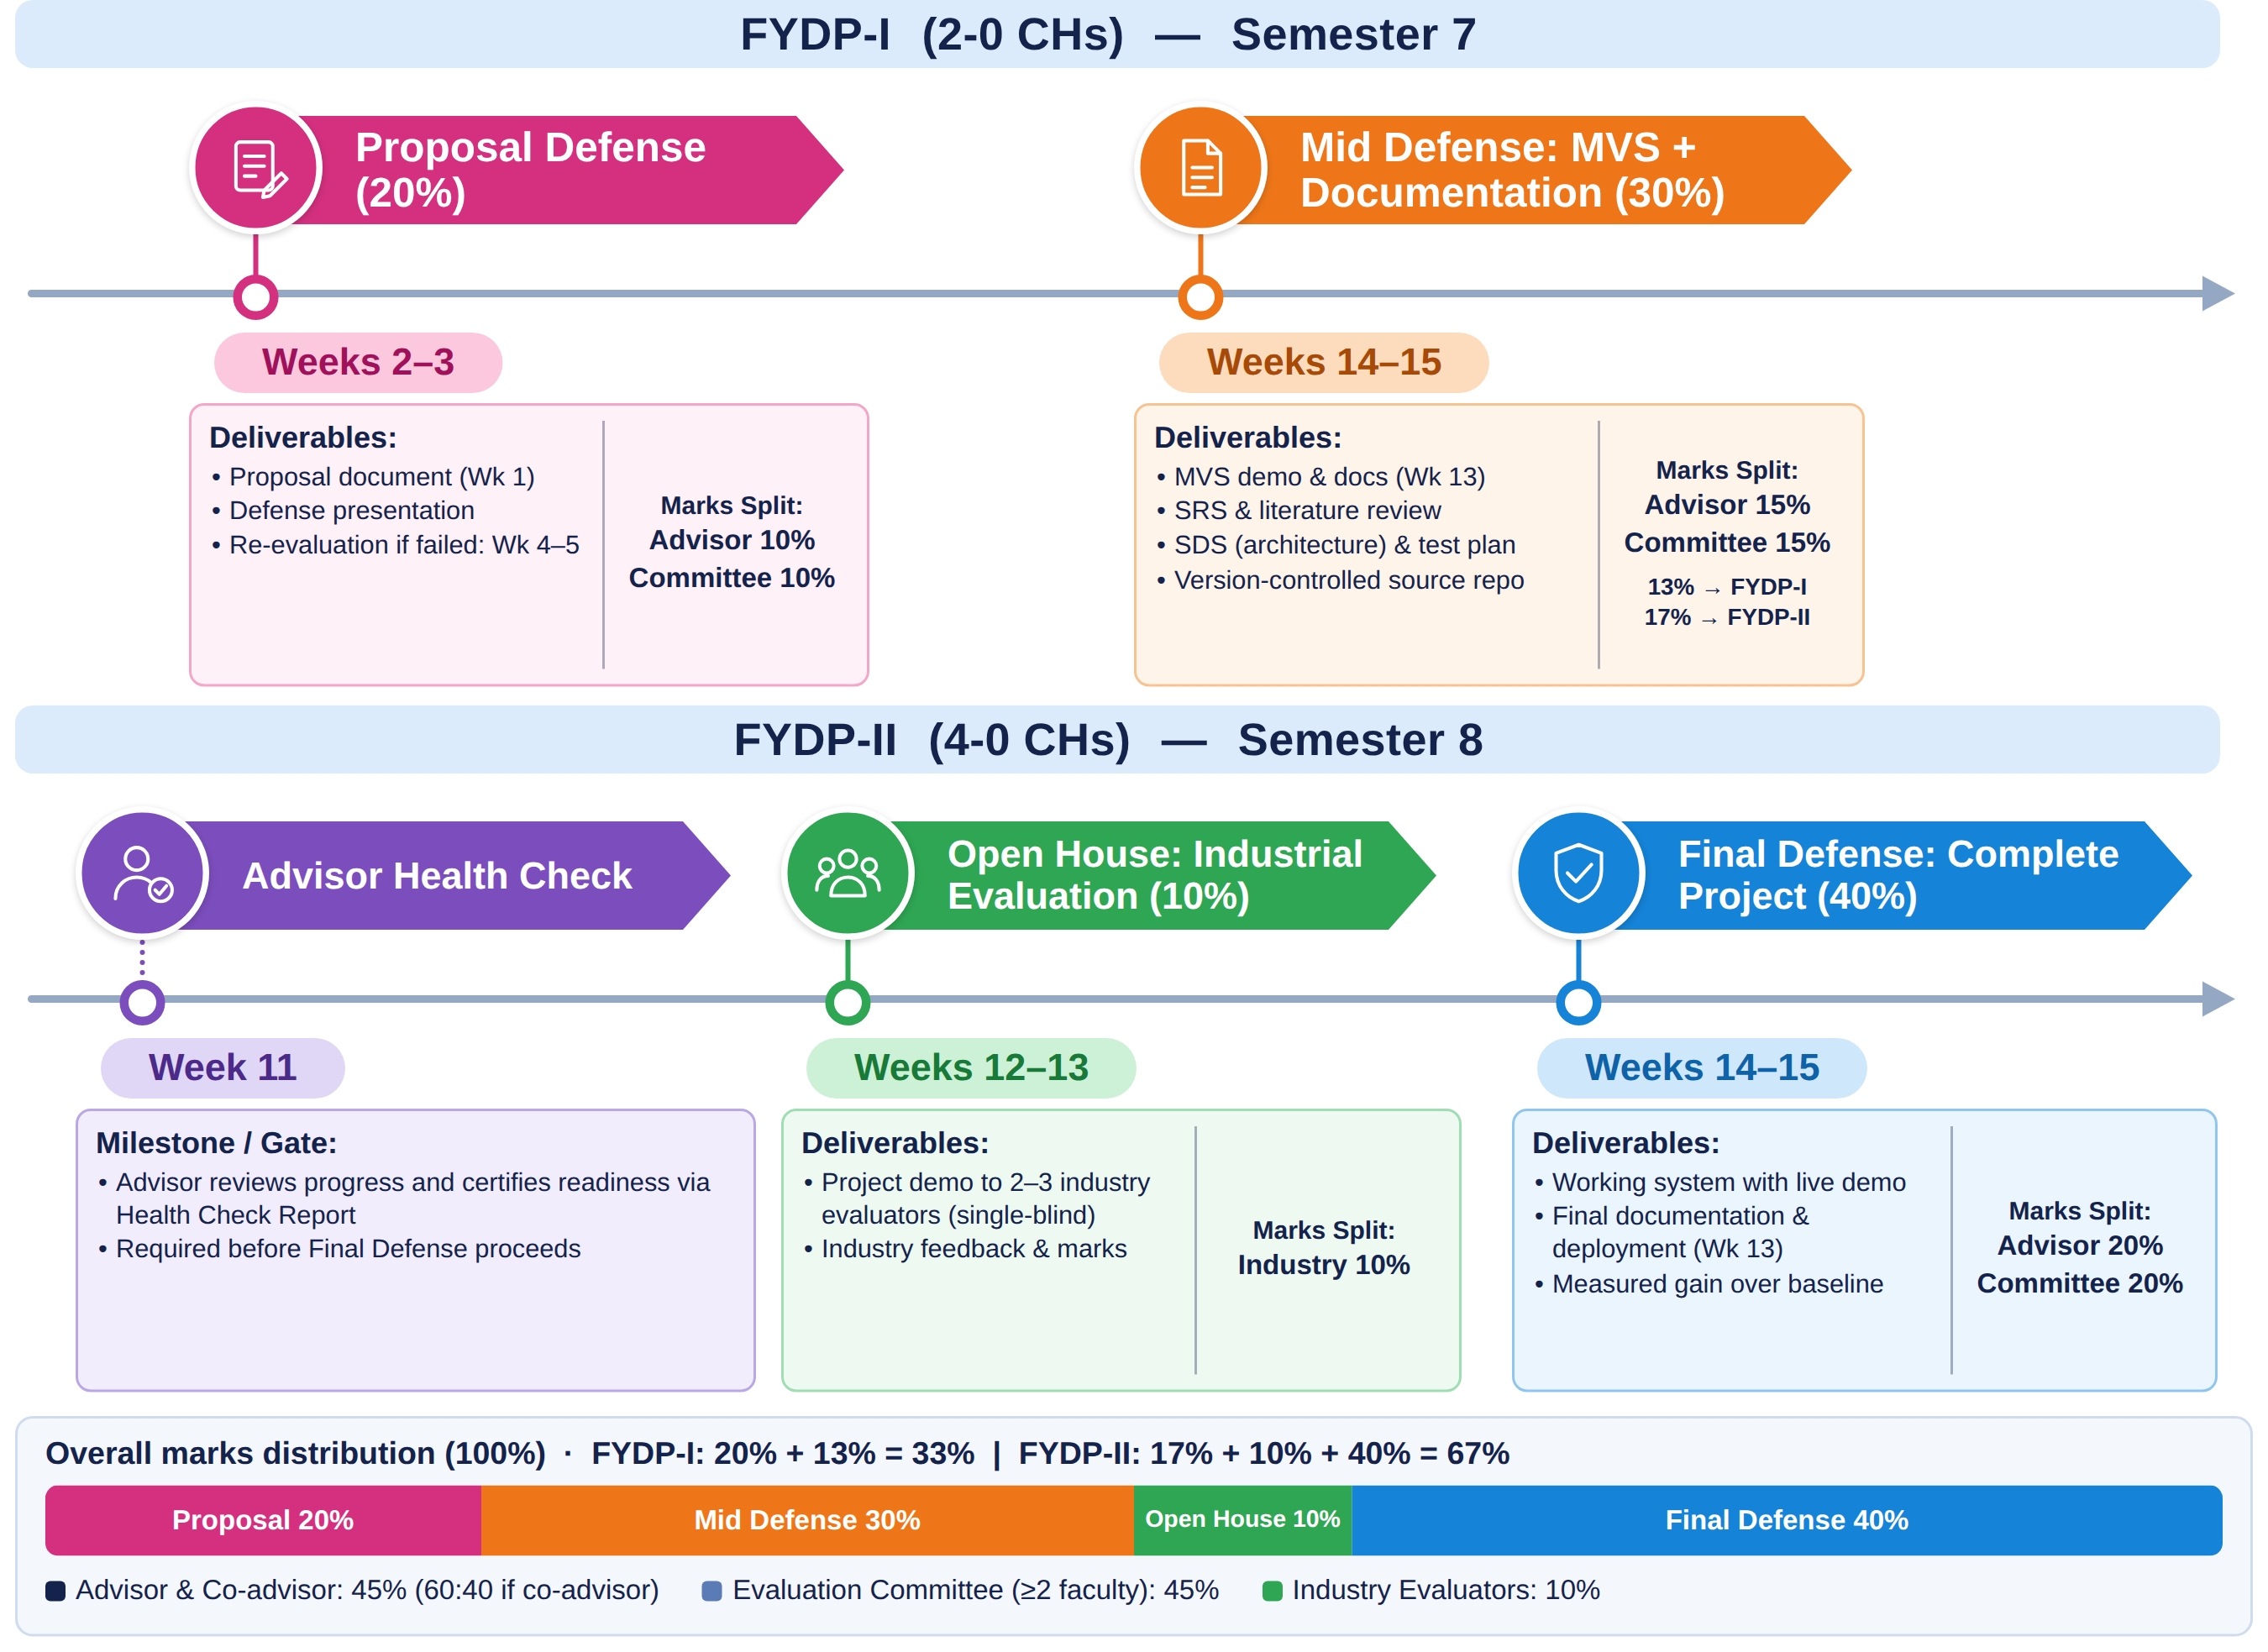
\includegraphics[width=1.0\textwidth]{images/criterion_2/media/FYDP-timeline.png}
\caption{Roadmap of Final Year Design Project (FYDP) Across 7\textsuperscript{th} \& 8\textsuperscript{th} Semesters.}
\label{figure:fydp}
\end{figure}
%-----------------------------------------------------------------------
\hypertarget{sec:fall2025results}{%
\subsection{CLO \& PLO Attainment Results for Fall 2025 Semester}\label{sec:fall2025results}}

\subsubsection{PLO Attainment at Cohort Level}

Results for Fall 2025 semester were prepared by the faculty using the OBE reports downloaded from the Qalam as mentioned in the previous sections. Data for cohort is extracted from the OBE reports and used for measurement of CLOs and PLOs attainment. The following section describe intake 2K23 batch results for attainment of CLOs and PLOs for Fall 2025 semester. The rest of the results of batch 2K22, 2K24, and 2K25 are provided in Annexure~\ref{annex:clo-plo-attainment-results}.

\paragraph{Fall 2025 Semester Results of Intake 2K23 Batch:} Figure~\ref{figure:2K23 Batch Result for All Courses} shows a screenshot of spreadsheet for all the courses taken by 2K23 batch in Fall 2025 semester. The figure contains CLO-PLO mapping and percentage of CLO attainment that is directly imported from the individual CLO and PLO attainment reports of each course from Qalam. Figure~\ref{figure:2K23 Batch cohort CLO attainment} shows same information as bar chart showing percentage attainment of corresponding CLOs against each course. Figure~\ref{figure:2K23 Batch Result for All Courses} also shows calculation of PLOs attainment as ``Ys'' as well as in percentage. The same information is given for PLO percentages and overall batch PLO attainment percentage in Figure~\ref{figure:2K23 Batch course-wise PLO attainment} and Figure~\ref{figure:2023 Batch cohort PLO attainment}, respectively. It can be seen that the cohort has successfully attained the concerned CLOs for each course. Similarly, the cohort PLOs have been attained as per set KPIs.


\begin{figure}[h]
\centering
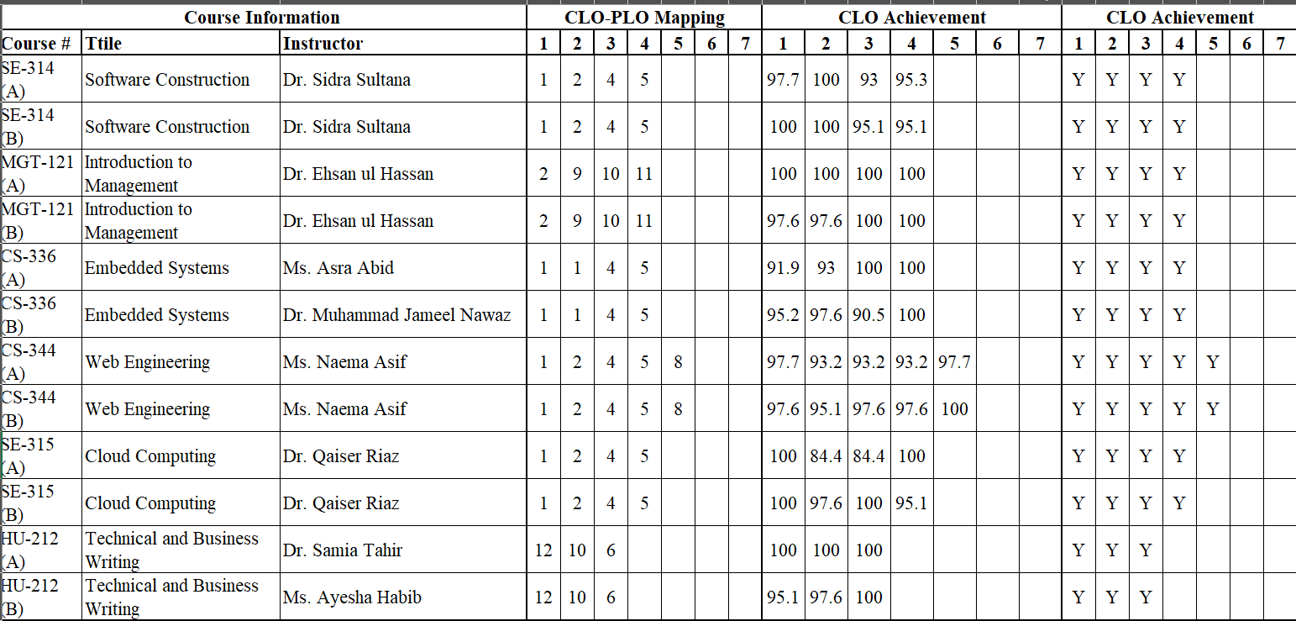
\includegraphics[width=0.98\linewidth]{images/criterion_2/media/image15.png}
\par\medskip
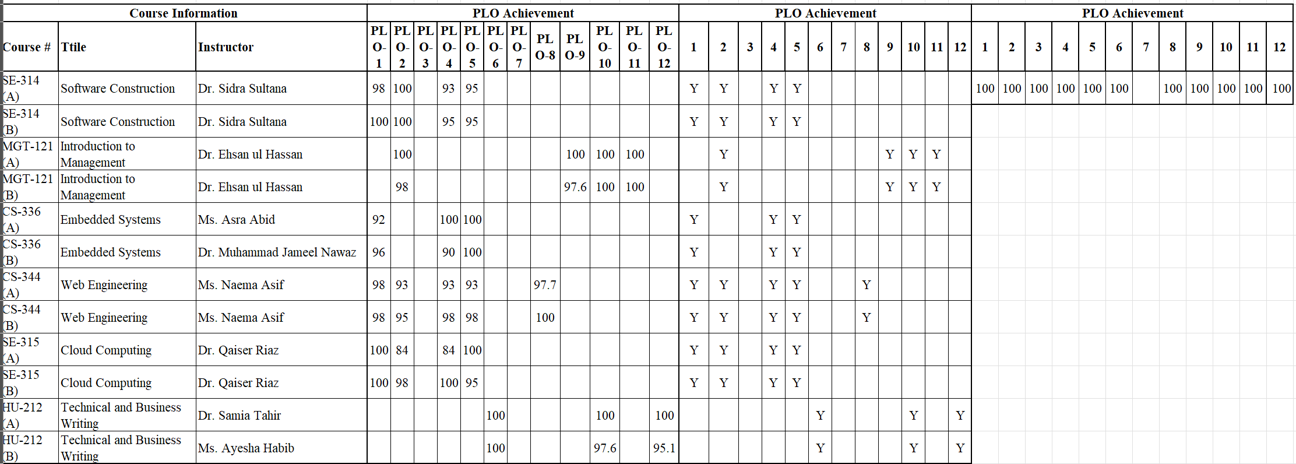
\includegraphics[width=0.98\linewidth]{images/criterion_2/media/image16.png}
\caption{2K23 Batch Result for All Courses in Fall 2025 Semester}
\label{figure:2K23 Batch Result for All Courses}
\end{figure}


\begin{figure}[H]
\centering
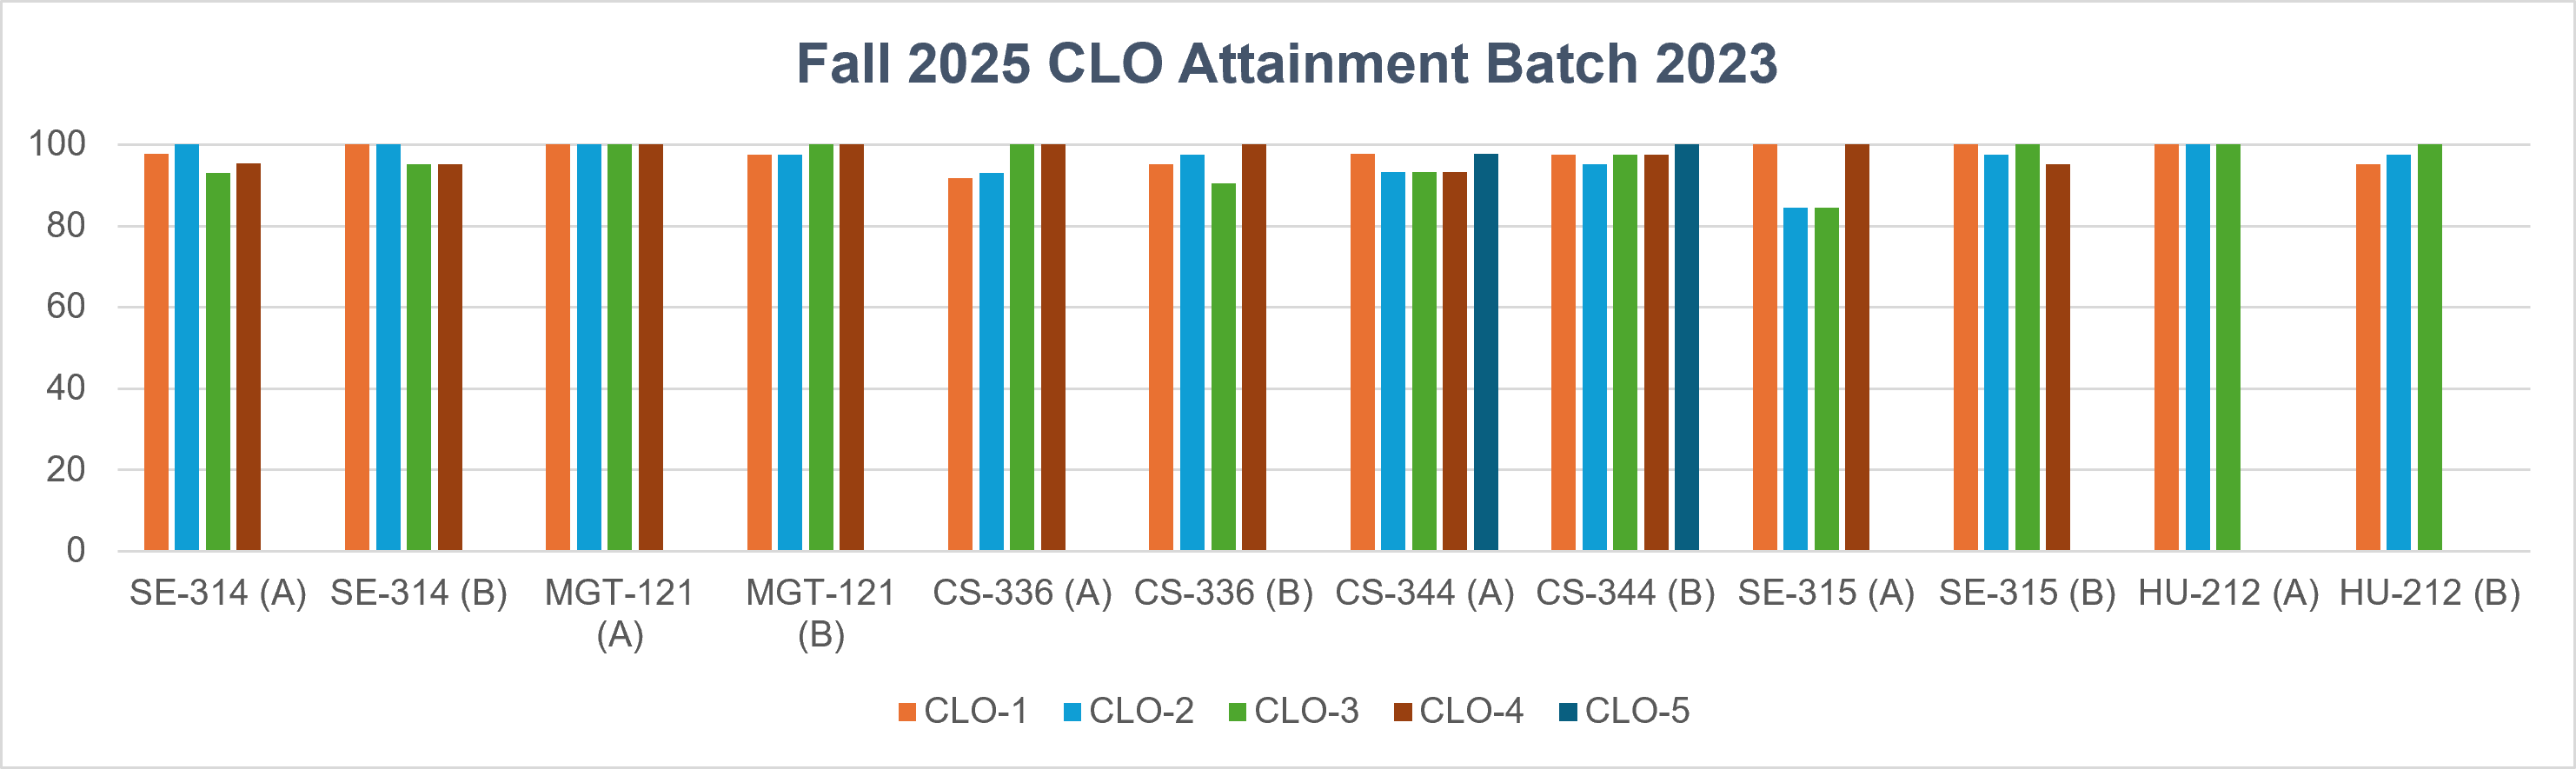
\includegraphics[width=0.97\textwidth]{images/criterion_2/media/image17.png}
\caption{2K23 Batch cohort CLO attainment for all courses in Fall 2025.}
\label{figure:2K23 Batch cohort CLO attainment}
\end{figure}

\begin{figure}[H]
\centering
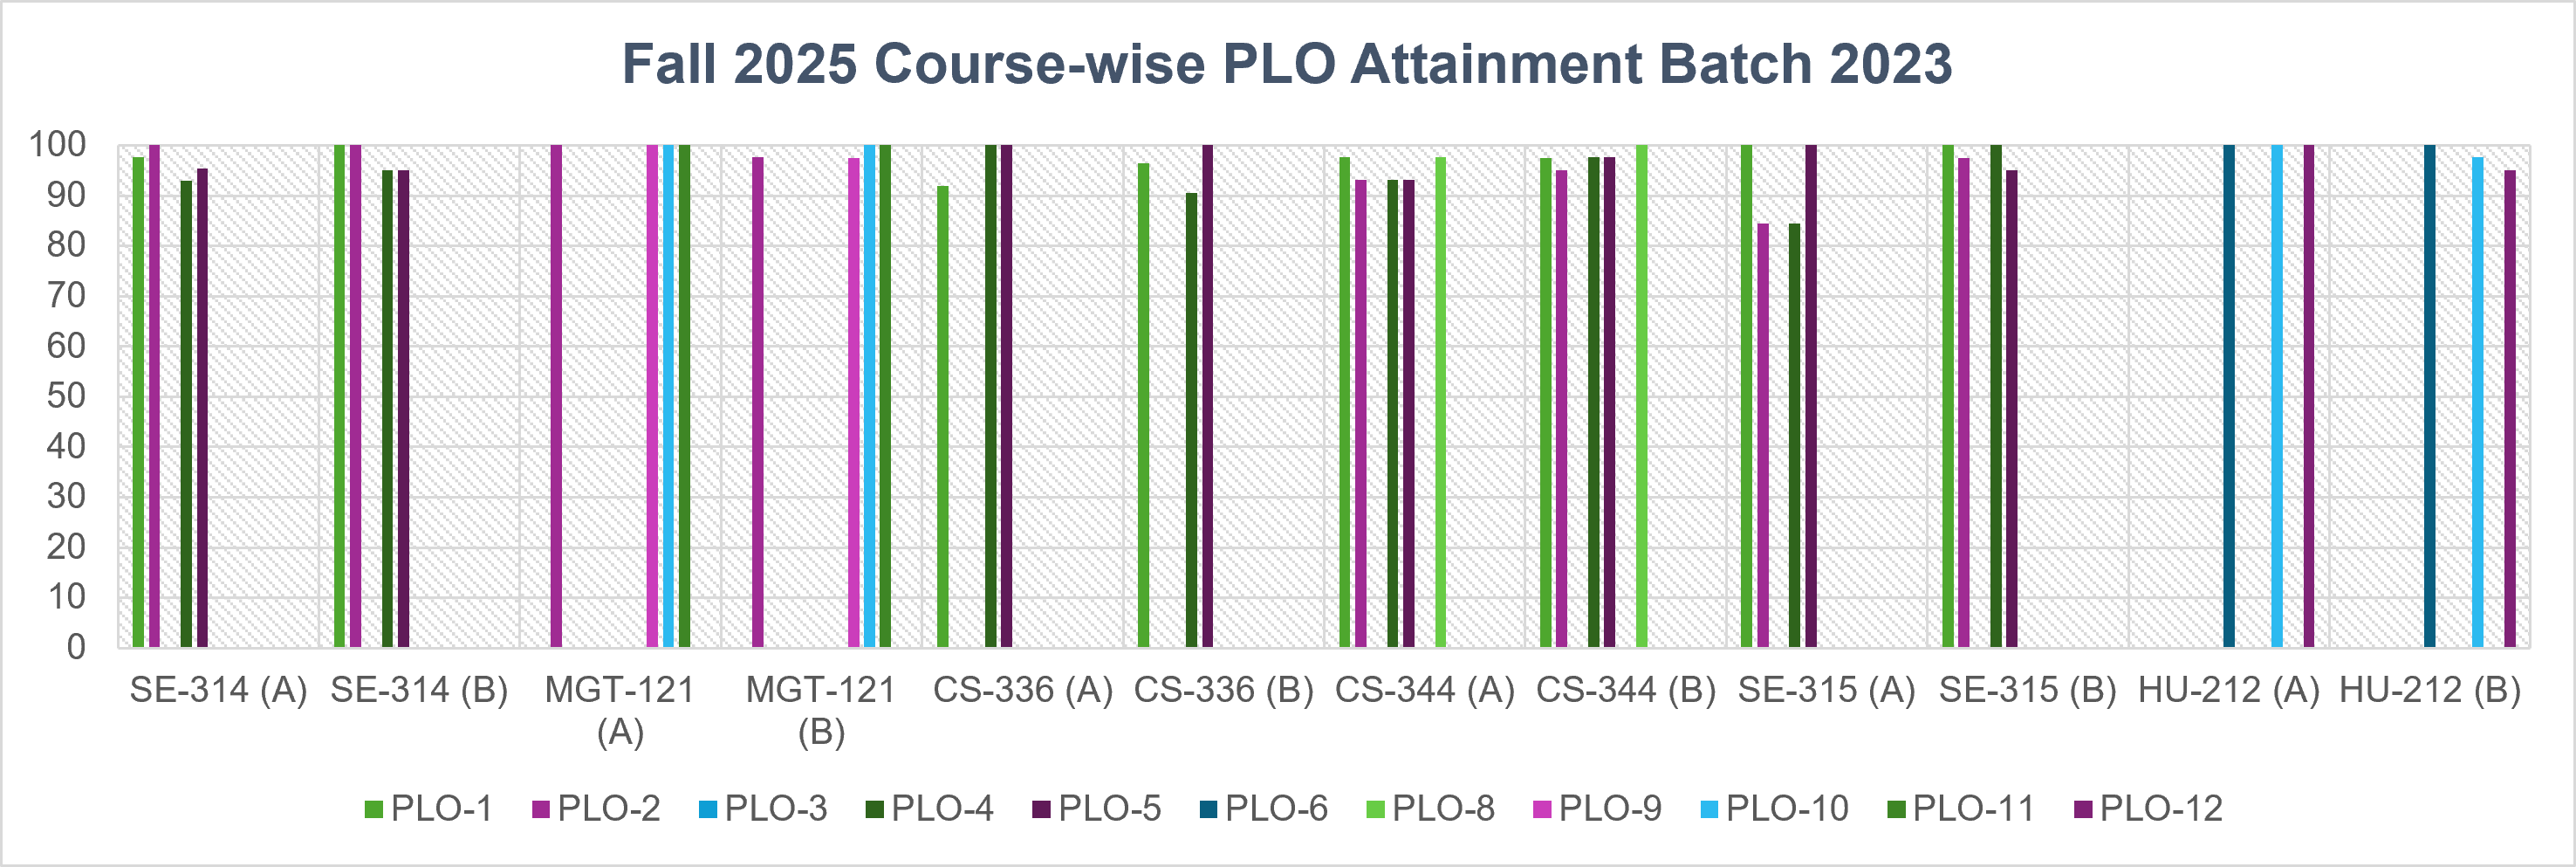
\includegraphics[width=0.98\textwidth]{images/criterion_2/media/image18.png}
\caption{2K23 Batch course-wise PLO attainment for Fall 2025.}
\label{figure:2K23 Batch course-wise PLO attainment}
\end{figure}

\begin{figure}[H]
\centering
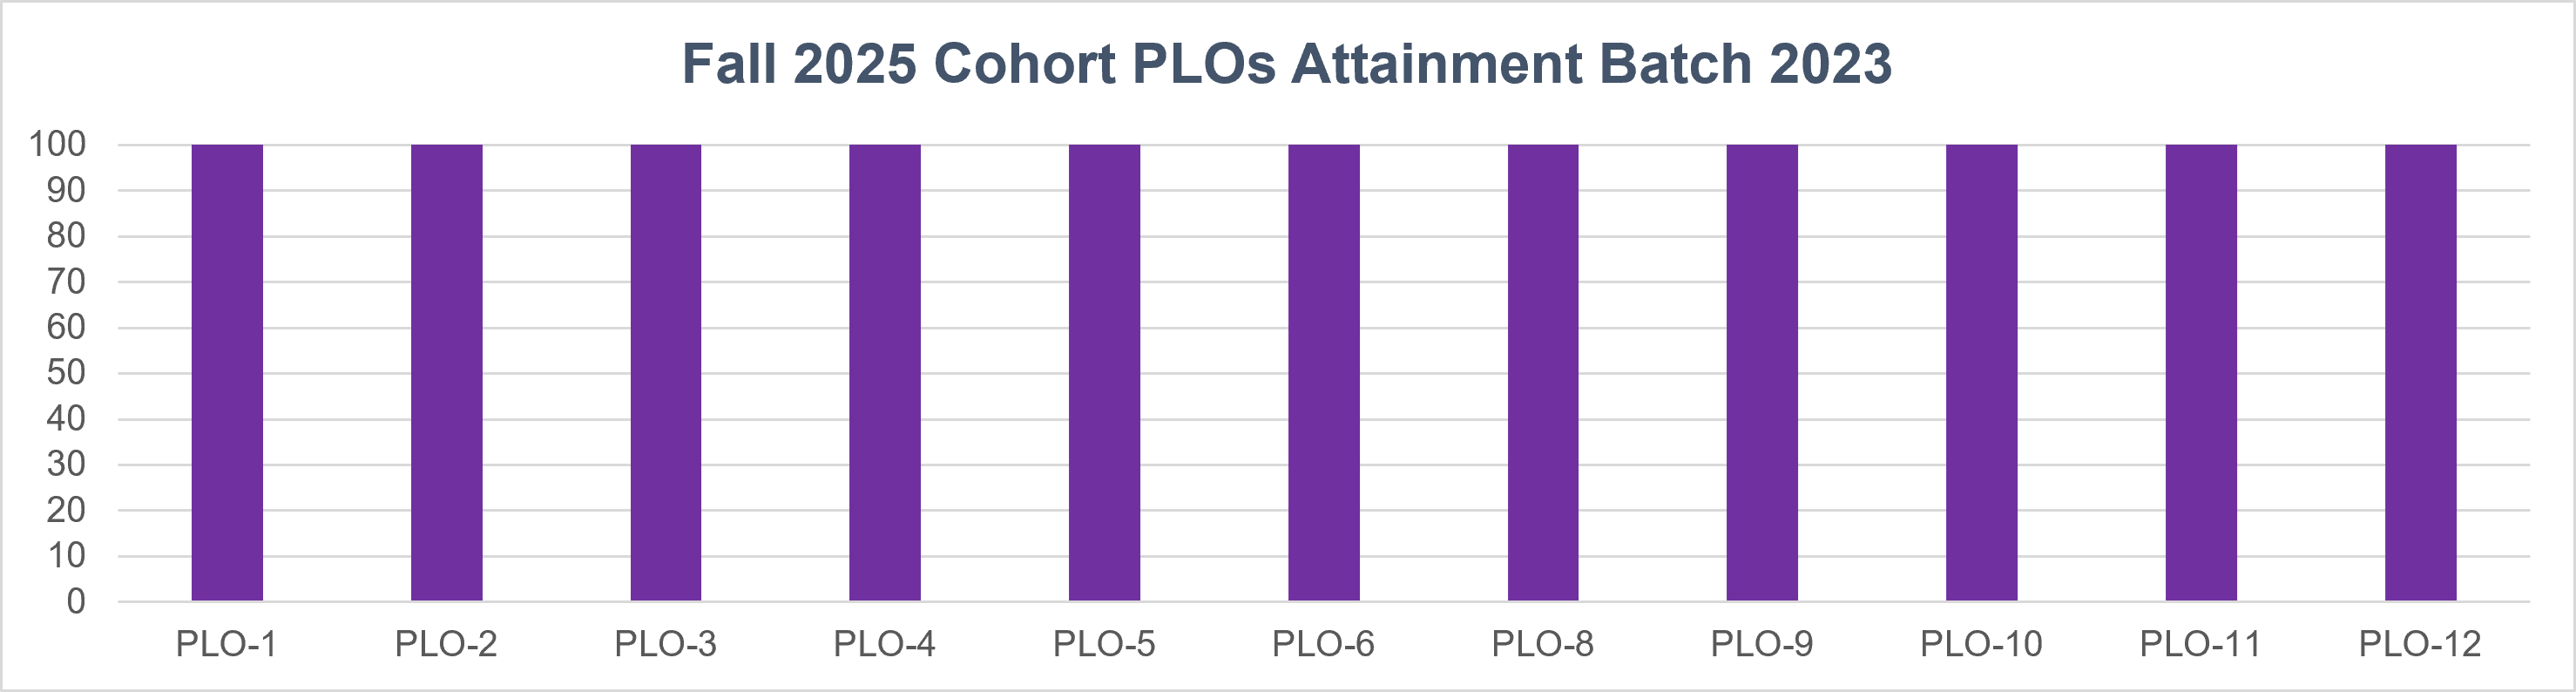
\includegraphics[width=0.98\textwidth]{images/criterion_2/media/image19.png}
\caption{2K23 Batch cohort PLO attainment against the 60\% KPI.}
\label{figure:2023 Batch cohort PLO attainment}
\end{figure}

\subsubsection{PLO Attainment at Individual Level}

Data from each course is forwarded to the exam branch which maintains a compilation of all courses for a particular batch. Data for each student is being maintained for PLOs as ``Y'' for PLOs attained by student and ``N'' for those not attained. A sample chart for a student showing attainment of PLOs is shown in Table~\ref{table:Cohort CLOs Attainment for CS-251}.

\clearpage
\begin{landscape}
\begingroup\scriptsize\setlength{\tabcolsep}{2pt}
\begin{longtable}{>{\raggedright\arraybackslash}p{0.10\linewidth}
                  >{\centering\arraybackslash}p{0.07\linewidth}
                  >{\raggedright\arraybackslash}p{0.18\linewidth}
                  >{\centering\arraybackslash}p{0.042\linewidth}
                  >{\centering\arraybackslash}p{0.042\linewidth}
                  >{\centering\arraybackslash}p{0.042\linewidth}
                  >{\centering\arraybackslash}p{0.042\linewidth}
                  >{\centering\arraybackslash}p{0.042\linewidth}
                  >{\centering\arraybackslash}p{0.042\linewidth}
                  >{\centering\arraybackslash}p{0.042\linewidth}
                  >{\centering\arraybackslash}p{0.042\linewidth}
                  >{\centering\arraybackslash}p{0.042\linewidth}
                  >{\centering\arraybackslash}p{0.050\linewidth}
                  >{\centering\arraybackslash}p{0.042\linewidth}
                  >{\centering\arraybackslash}p{0.042\linewidth}}
\caption{PLOs Attainment for an Individual Student. Student Name: Muhammad Sohaib Akhtar, Registration No.: 456318 (2023 Batch)} \\
\toprule
\textbf{Semester} & \textbf{Code} & \textbf{Course Title} & \textbf{PLO-1} & \textbf{PLO-2} & \textbf{PLO-3} & \textbf{PLO-4} & \textbf{PLO-5} & \textbf{PLO-6} & \textbf{PLO-7} & \textbf{PLO-8} & \textbf{PLO-9} & \textbf{PLO-10} & \textbf{PLO-11} & \textbf{PLO-12} \\
\midrule
\endfirsthead
\multicolumn{15}{l}{\footnotesize\textit{Continued from previous page}} \\
\toprule
\textbf{Semester} & \textbf{Code} & \textbf{Course Title} & \textbf{PLO-1} & \textbf{PLO-2} & \textbf{PLO-3} & \textbf{PLO-4} & \textbf{PLO-5} & \textbf{PLO-6} & \textbf{PLO-7} & \textbf{PLO-8} & \textbf{PLO-9} & \textbf{PLO-10} & \textbf{PLO-11} & \textbf{PLO-12} \\
\midrule
\endhead
\midrule\multicolumn{15}{r}{\footnotesize\textit{Continued on next page}} \\
\endfoot
\bottomrule
\endlastfoot
\textbf{1 (Fall-2023)} & CS-110   & Fundamentals of Computer Programming & Y & & Y & & Y & & & & Y & & & \\
 & HU-107   & Pakistan Studies                    &   &   &   &   &   & Y &   & Y &   &   &   & Y \\
 & HU-110   & English                             &   &   &   &   &   &   &   &   &   & Y &   & Y \\
 & MATH-101 & Calculus \& Analytical Geometry     & Y & \cellcolor{Red!20}{N} &   &   &   &   &   &   &   &   &   &   \\
 & MATH-161 & Discrete Mathematics                & Y & Y & Y &   &   &   &   &   &   &   &   &   \\
 & OHS-101  & Occupational Health and Safety      &   &   &   &   &   & Y & Y &   &   &   &   &   \\
 & PHY-102  & Applied Physics                     & Y & Y &   &   &   &   &   &   &   &   &   &   \\
\textbf{2 (Spr.-2024)} & CS-212  & Object Oriented Programming         & Y & Y & Y &   & Y &   &   & Y &   &   &   &   \\
 & EE-122   & Computer Architecture and Logic Design & Y & Y & Y & Y & Y &  &  & Y & Y &  &  &  \\
 & HU-101   & Islamic Studies                     &   &   &   &   &   & Y &   & Y &   &   &   & Y \\
 & HU-109   & Communication Skills                &   &   &   &   &   &   &   & Y &   & Y &   & Y \\
 & MATH-121 & Linear Algebra \& ODEs              & Y & Y &   &   &   &   &   &   &   &   &   &   \\
 & ME-105   & Workshop Practice                   & Y &   & Y &   &   &   &   &   & Y &   &   &   \\
 & ME-109   & Engineering Drawing                 & Y &   &   &   & Y &   &   &   &   &   &   &   \\
\textbf{3 (Fall-2024)} & CS-220  & Database Systems                     & Y &   & Y & Y & Y &   &   &   &   &   &   &   \\
 & CS-250   & Data Structures and Algorithms      & Y & Y &   &   & Y &   &   & Y & Y &   &   &   \\
 & EE-353   & Computer Networks                   & Y &   & Y & Y & Y &   &   &   &   &   &   &   \\
 & MATH-352 & Numerical Methods                   & Y & Y &   &   & Y &   &   &   &   &   &   &   \\
 & SE-200   & Software Engineering                & Y & Y & Y & Y &   &   &   &   & Y &   &   &   \\
\textbf{4 (Spr. 2025)} & CS-251  & Design \& Analysis of Algorithm      &   & Y & Y & Y &   &   &   &   &   &   &   &   \\
 & CS-330   & Operating Systems                   & Y & Y &   & Y & Y &   &   &   &   &   &   &   \\
 & HU-222   & Professional Ethics                 &   &   &   &   &   & Y &   & Y &   &   &   & Y \\
 & MATH-232 & Complex Variables and Transforms    & Y & Y & Y &   &   &   &   &   &   &   &   &   \\
 & MATH-361 & Probability \& Statistics           & Y & Y & Y &   &   &   &   &   &   &   &   &   \\
 & SE-211   & Software Design and Architecture    & Y & Y & Y & Y &   &   &   &   &   &   &   &   \\
\textbf{5 (Fall-2025)} & CS-336  & Embedded Systems                     & Y &   &   & Y & Y &   &   &   &   &   &   &   \\
 & CS-344   & Web Engineering                     & Y & Y &   & Y & Y &   &   &   & Y &   &   &   \\
 & HU-212   & Technical \& Business Writing       &   &   &   &   &   & Y &   &   &   & Y &   & Y \\
 & MGT-121  & Introduction To Management          &   & Y &   &   &   &   &   &   &   & Y & Y & Y \\
 & SE-314   & Software Construction               & Y & Y & Y &   & Y &   &   &   &   &   &   &   \\
 & SE-315   & Cloud Computing                     & Y & Y &   & Y & Y &   &   &   &   &   &   &   \\
\textbf{6 (Spr.-2026)} & CS-261  & Human Computer Interaction & \multicolumn{12}{l}{\textit{Spring 2026 semester in progress}} \\
 & SE-320   & Formal Methods                      & \multicolumn{12}{l}{} \\
 & SE-430   & Software Project Management         & \multicolumn{12}{l}{} \\
 & CS-471   & Machine Learning                    & \multicolumn{12}{l}{} \\
 & SE-321   & Software Quality Engineering        & \multicolumn{12}{l}{} \\
 & MGT-271  & Entrepreneurship                    & \multicolumn{12}{l}{} \\
\end{longtable}
\endgroup
\end{landscape}

%-----------------------------------------------------------------------
\hypertarget{sec:representative-course}{%
\subsection{Representative Course Result for Attainment of CLOs and PLOs}\label{sec:representative-course}}

A representative course CS-251 Design and Analysis of Algorithms, taken by 2024 batch as a core course in Spring 2026 semester is presented here to show the entire process of assessment at course level and calculations of results for attainment of CLOs as well as the PLOs. The CLO and PLO attainment report is given in Annexure~\ref{Sample CLO Attainment Report} and Annexure~\ref{Sample PLO Attainment Report}. The results for the cohort are tabulated in Table~\ref{table:Cohort CLOs Attainment for CS-251} for CLOs attainment and in Table~\ref{table:Cohort PLOs Attainment for CS-251} for PLOs attainment. Out of 45 students the percentage attainment for CLO-1, CLO-2 and CLO-3 were recorded as $91.11\%$, $91.11\%$ and $80$, respectively for the course. Figure~\ref{figure:Cohort CLO-PLO attainment Histogram} shows percent attainment of CLOs and PLOs for the entire course. The course was reviewed by the LQEC and according to OBE framework manual, attainment of all the CLOs is well above the set cohort KPI of 60\% depicting none of the corrective actions to be undertaken.

\begin{table}[H]
\centering
\caption{Cohort CLOs Attainment for CS-251 Design \& Analysis of Algorithms}
\footnotesize
\begin{tabular}{>{\raggedright\arraybackslash}p{0.50\textwidth}
                >{\centering\arraybackslash}p{0.12\textwidth}
                >{\centering\arraybackslash}p{0.12\textwidth}
                >{\centering\arraybackslash}p{0.12\textwidth}}
\toprule
\multicolumn{4}{l}{\textbf{Cohort KPI for CQI = 60\% Students Pass CLO (CLO $\geq$ 50\%)}} \\
\midrule
 & \textbf{CLO-1} & \textbf{CLO-2} & \textbf{CLO-3} \\
Total Students Attaining CLO & 41/45 & 41/45 & 36/45 \\
Percentage Students Attaining CLO & 91.11\% & 91.11\% & 80\% \\
CLO Attainment & Yes & Yes & Yes \\
\bottomrule
\end{tabular}
\label{table:Cohort CLOs Attainment for CS-251}
\end{table}

\begin{table}[H]
\centering
\caption{Cohort PLOs Attainment for CS-251 Design \& Analysis of Algorithms}
\footnotesize
\begin{tabular}{>{\raggedright\arraybackslash}p{0.50\textwidth}
                >{\centering\arraybackslash}p{0.12\textwidth}
                >{\centering\arraybackslash}p{0.12\textwidth}
                >{\centering\arraybackslash}p{0.12\textwidth}}
\toprule
\multicolumn{4}{l}{\textbf{Cohort KPI for CQI = 60\% Students Pass PLO (PLO $\geq$ 50\%)}} \\
\midrule
 & \textbf{PLO-2} & \textbf{PLO-3} & \textbf{PLO-4} \\
Total Students Attaining PLO & 41/45 & 41/45 & 36/45 \\
\%age Students Attaining PLO & 91.11\% & 91.11\% & 80\% \\
PLO Attainment & Yes & Yes & Yes \\
\bottomrule
\end{tabular}
\label{table:Cohort PLOs Attainment for CS-251}
\end{table}

\begin{figure}[H]
\centering
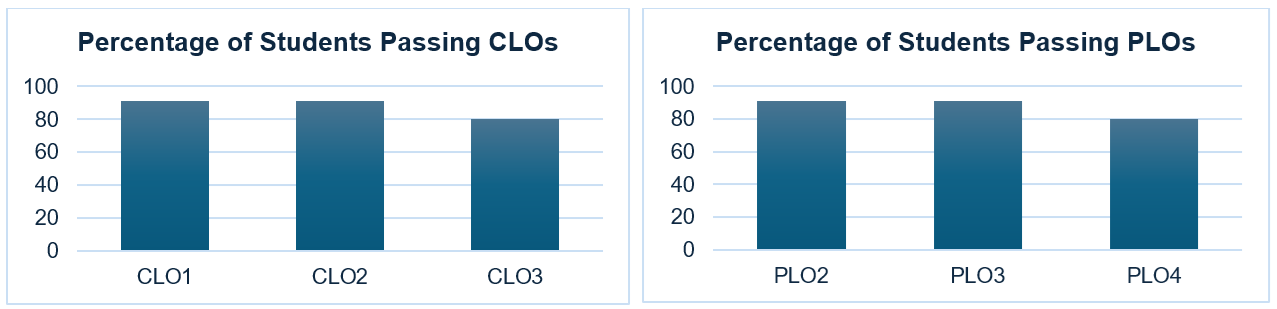
\includegraphics[width=0.99\textwidth]{images/criterion_2/media/image22.png}
\caption{Cohort CLO \& PLO attainment for CS-251 Design and Analysis of Algorithms}
\label{figure:Cohort CLO-PLO attainment Histogram}
\end{figure}

%\begin{figure}[H]
%\centering
%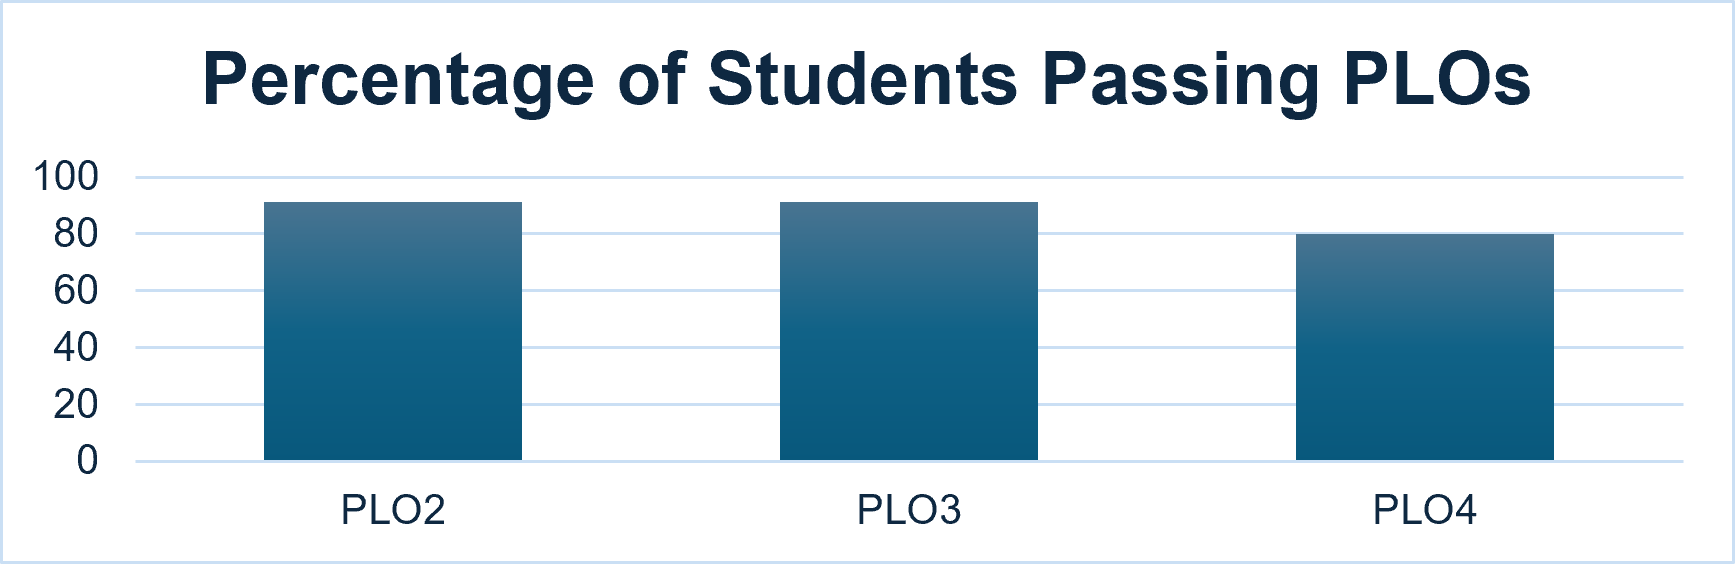
\includegraphics[width=0.86\textwidth]{images/criterion_2/media/image21.png}
%\caption{Cohort PLO attainment for CS-251 Design and Analysis of Algorithms, 2024 Batch.}
%\label{figure:Cohort PLO attainment Histogram}
%\end{figure}


%-----------------------------------------------------------------------
\hypertarget{sec:indirectassess}{%
\section{Indirect PLO Assessment}\label{sec:indirectassess}}

This method of assessment is accomplished through internship feedback and exit surveys.

\subsection{Internship Feedback}\label{sec:internshipfeedback}

Students of BESE program are required to complete their internships preferably during the summer semester. The internship feedback is obtained at the end of summer semester in their second/third year. The details of internship program are given in Chapter~\ref{criterion3}, Section~\ref{sec:4.8internship} Internship Program. The existing forms for internship feedback were revised to obtain indirect assessment of PLOs from employers of the internees. The sample internship feedback form is given in Annexure~\ref{annex:internship-feedback-form}. In the Annexure~\ref{annex:internship-feedback-analysis}, a detailed analysis of PLO attainment through internship feedback for 2K21, 2k22 and 2K23 batches is provided.

The internship feedback from employers provides indirect evidence of PLO attainment for BESE batches 2K21, 2K22, and 2K23. Overall, the results demonstrate consistently positive employer perceptions, with the majority of ratings concentrated at 4 (Very Good) and 5 (Excellent) and negligible negative ratings. Across the three batches, PLO 1 (Engineering Knowledge), PLO 11 (Project Management), and PLO 12 (Lifelong Learning) consistently emerged among the strongest attributes, indicating that graduates demonstrate sound technical foundations, effective decision-making, professional maturity, willingness to learn, and receptiveness to feedback in workplace environments.

The comparative analysis also identifies areas for continued improvement. For batches 2K21 and 2K22, PLO 2 (Problem Identification and Analysis), PLO 3 (Design and Development), and PLO 7 (Environment and Sustainability) show relatively lower proportions of Excellent ratings, although the combined Very Good and Excellent ratings remain strong. PLO 8 (Ethics) and PLO 9 (Individual and Teamwork) similarly show a strong overall performance but provide opportunities for further development. The 2K23 results, although based on interim and comparatively smaller data, show a highly positive trend, with most PLOs achieving over 90\% combined ratings of 4 and 5. Overall, the three-batch comparison indicates that the BESE program is effectively developing competencies valued by industry, while the identified areas of comparatively lower attainment provide useful input for the CQI process. The findings can therefore be used to strengthen curriculum content, practical and design-oriented activities, professional skills development, and industry exposure, particularly in complex problem-solving, system design, sustainability, and workplace professionalism.

\subsection{Exit Survey}

The exit survey seeks graduating students input on quality of education they received during their program. The purpose of this survey is to assess the perception of graduating students on achievement of PLOs. Sample of the exit survey form is given in Annexure~\ref{annex:graduate-exit-survey-form}.

The Graduate Exit Survey provides indirect evidence of PLO attainment through graduating students’ self-assessment on a 5-point Likert scale. The results for batches 2K20, 2K21, and 2K22 demonstrate consistently positive attainment across all 12 PLOs, with mean scores generally close to or above 4.0. The 2K20 batch showed a particularly stable performance, with students expressing strong confidence in lifelong learning, communication, and professional competencies. The 2K21 batch similarly demonstrated strong performance, particularly in ethics, teamwork, communication, and engineering and societal considerations.

The 2K22 batch maintained a positive overall profile, with teamwork (PLO 9), lifelong learning (PLO 12), and communication (PLO 10) emerging as the strongest areas. Across the batches, some variation was observed in students’ perceptions of engineering knowledge, problem analysis, design and development, modern tool usage, and professional ethics, providing useful areas for further attention. In particular, the relatively lower scores for PLO 8 and PLO 5 in 2K22 indicate opportunities to further strengthen ethical responsibility, accountability, and hands-on familiarity with evolving industry tools.

Overall, the exit survey results indicate that graduates perceive themselves as well prepared in both technical and professional competencies, with strong capabilities in communication, teamwork, ethical/professional conduct, management, and lifelong learning. The identified areas of relatively lower attainment are used as input to the CQI process to further enhance curriculum content, practical exposure, assessment strategies, and professional development activities. The detailed analysis of graduate exit survey is provided in Annexure~\ref{annex:graduate-exit-survey-analysis}. 

%-----------------------------------------------------------------------
\hypertarget{sec:application}{%
\section{Application of Assessment Results for Improvement of Program}\label{sec:application}}

LQEC evaluates results of the course in consultation with the concerned faculty and HoD for any recommended improvements. If some deficiency is identified through CQI, the corrective action process is invoked by the LQEC. The process for corrective action identifies the nature of problems that may be improved through review process as described in Section~\ref{sec:cqiplos}. If the weakness is related to achievement of CLOs and/or PLOs through coursework, the revision of curriculum or other corrective actions are recommended. The possible corrective actions may be, the revision of curriculum, redefining of CLOs, revision of CLOs to PLOs mapping, the assessment methods, instruction methodology, or mentoring/training of faculty.

\hypertarget{sec:cqiclos}{%
\subsection{Review and Corrective Action Process for Course (CLOs)}\label{sec:cqiclos}}

The CQI process for CLOs at SEECS is a robust, institutionalized mechanism designed to ensure that academic offerings remain rigorous, current, and tightly aligned with PLOs. Rather than being isolated or ad-hoc, CQI operates through a well-defined institutional lifecycle that guarantees traceability, formal governance review, and systematic monitoring. Figure~\ref{CLo-CQI} shows the CQI process of CLOs.

\begin{figure}[H]
\centering
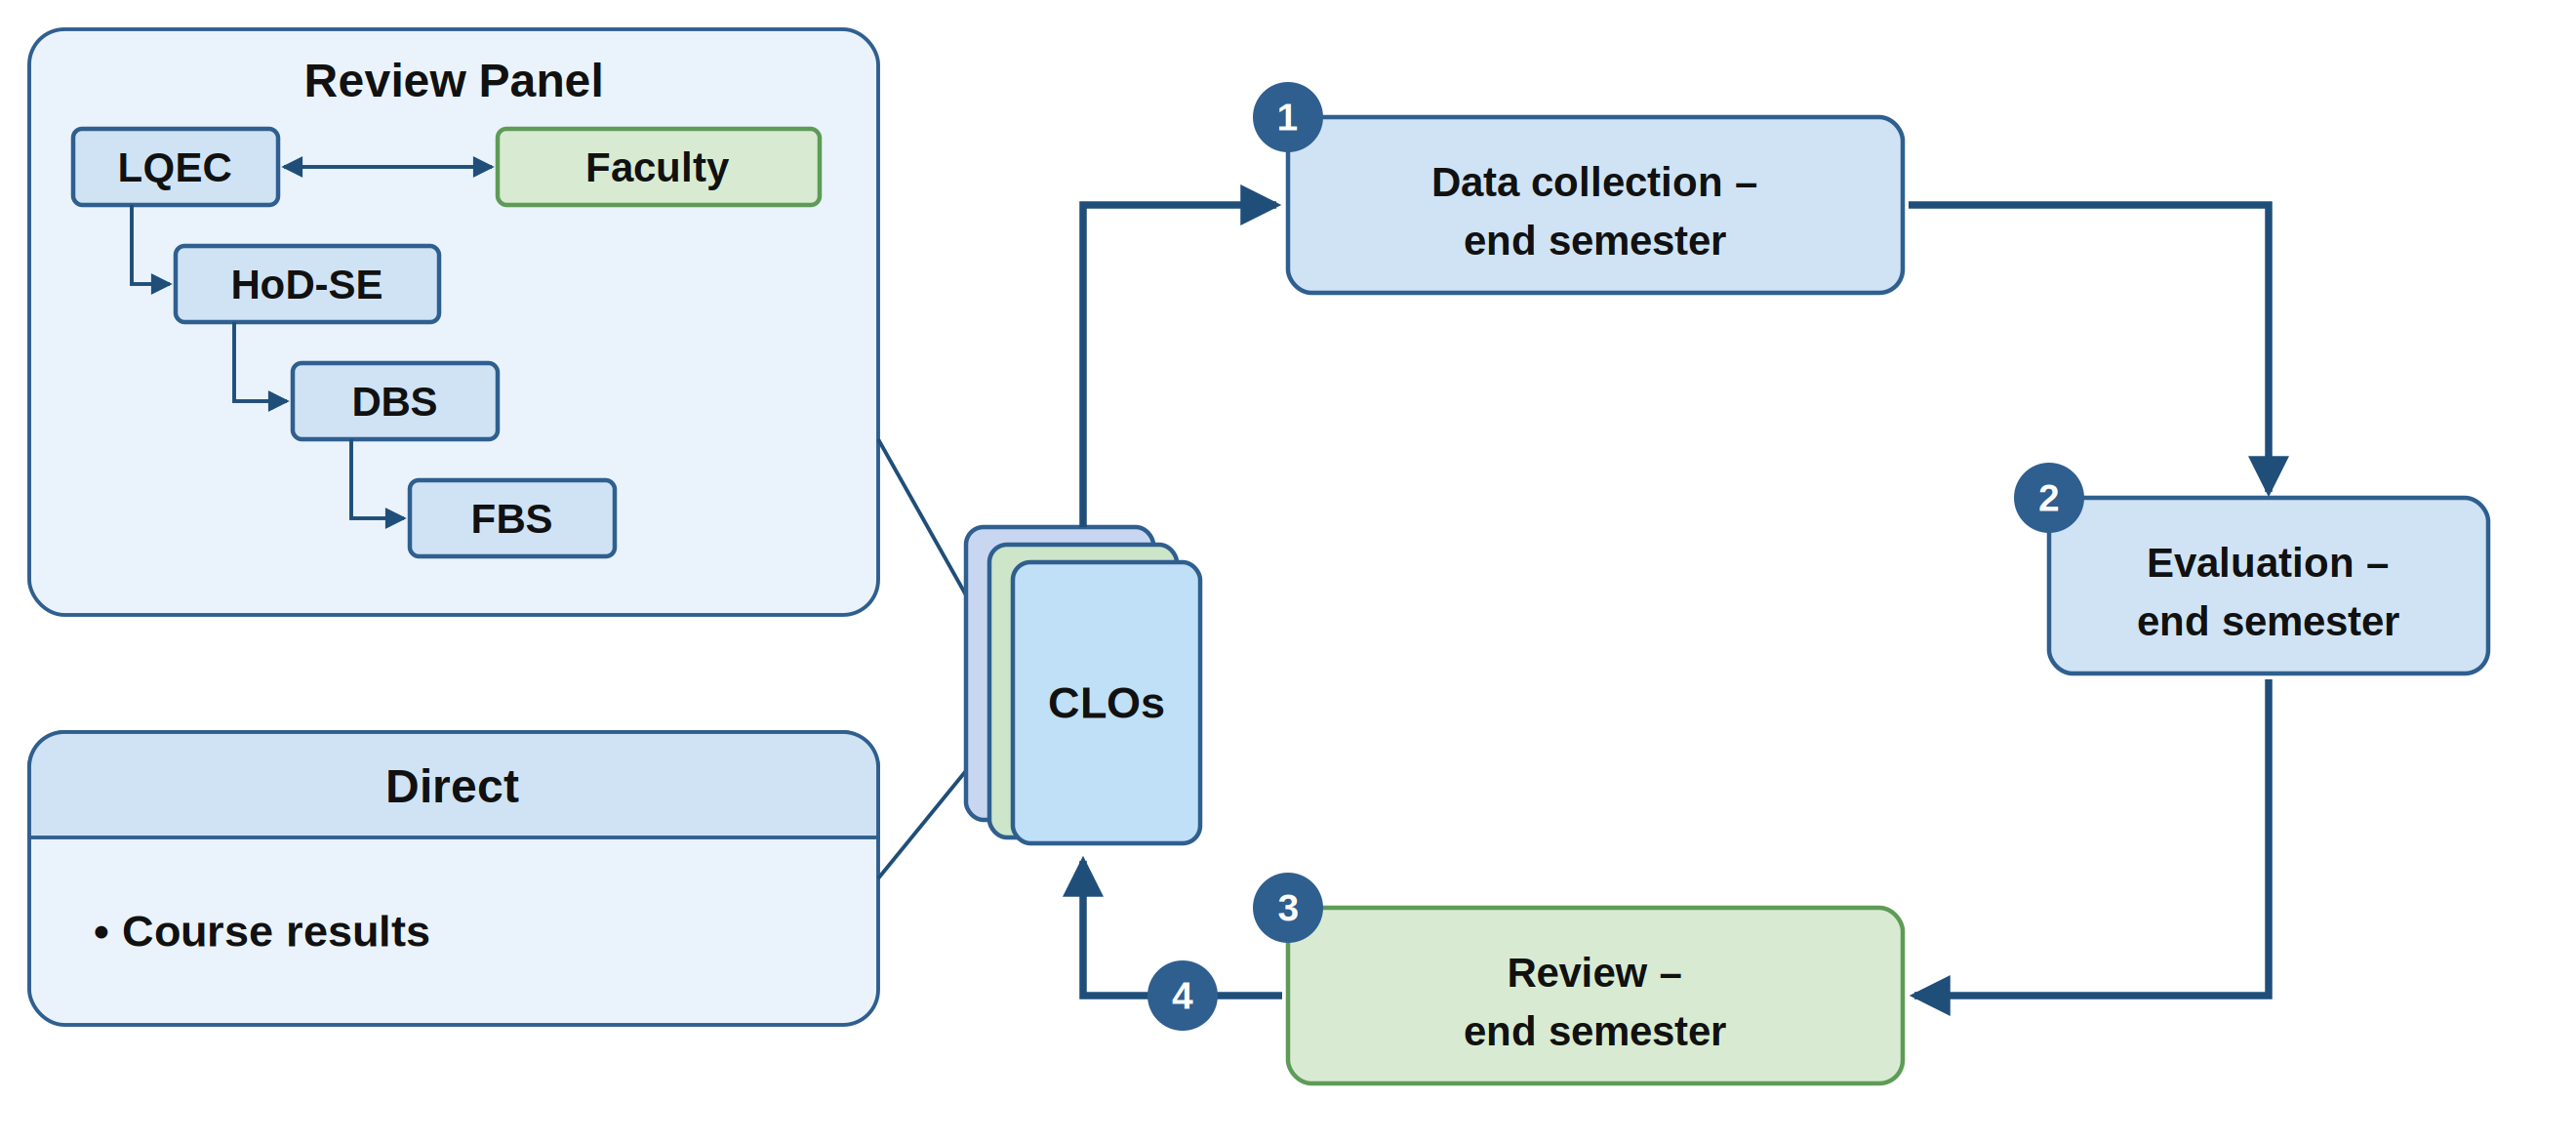
\includegraphics[width=0.9\textwidth]{images/front_matter/media/image-18.png}
\caption{Overview of the Processes Involved for Attainment and Review of CLOs.}
\label{CLo-CQI}
\end{figure}

The process universally begins with a formal identification phase, where HoD, Knowledge Group Heads (KGHs), or instructors recognize curricular deficiencies, such as misaligned CLOs, inappropriate Bloom's Taxonomy levels, outdated content, or pedagogical inconsistencies across different sections. Once an issue is identified, it is never addressed informally. Instead, it triggers a structured CQI and deliberation phase. The relevant Knowledge Group convenes to analyze the pedagogical gaps, redefine course scopes, rationalize CLO statements, and recalibrate BT levels to meet established educational benchmarks.

To demonstrate strict institutional rigor, all findings, justifications, and proposed remedies are formally captured using the Corrective Action Form (CAF). The sample corrective action form is provided in Annexure~\ref{annex:caf}. This document acts as an audit trail detailing the precise nature of the problem, the assessment of the issue, and the suggested corrective actions. Following documentation, the proposed changes cannot be implemented unilaterally. They must navigate a formal multi-tier governance structure for institutional approval. Proposed course outlines, revised CLO mappings, and curriculum updates are presented to higher academic forums such as the DBS for rigorous peer review and formal approval. Furthermore, mandatory institutional sign-offs from the LQEC, the UG Program Coordinator, and the Head of the Department validate the process before adoption. Once approved, the changes are strictly implemented in the subsequent semester, with LQEC actively monitoring execution to ensure consistent course delivery, proper assessment alignment, and improved outcome attainment. To see this institutionalized CQI process rigorously followed in practice, the curriculum review and modification for CS-212 Object-Oriented Programming (OOP) serves as a clear exemplar. The issue was formally flagged on January 31, 2024, when the Programming Core Knowledge Group identified the need to rationalize CLOs and unify programming language content across all sections of CS-212 to maintain a consistent standard of student expertise. To conduct the CQI, the Knowledge Group convened to evaluate the course structure, determining that the course would emphasize abstract OOP concepts reinforced through practical implementation in Java as a pure object-oriented language. They comprehensively updated the CLO statements, re-sequenced them, and aligned them with appropriate Bloom's Taxonomy levels and PLOs, such as upgrading CLO 2 to focus on evaluating complex programming problems at the C-5 level. This entire corrective plan was rigorously documented on an official Corrective Action Form (given in Annexure~\ref{annex:caf-oop}). Providing absolute institutional transparency and adherence to governance, the LQEC formally presented the updated course outline and revised CLOs to the DBS during its meeting on February 2, 2024 (given in Annexure~\ref{annex:dbs-mom}). The DBS formally approved the curriculum changes. The revised framework complete with updated CLOs, mapped teaching methods, and week-by-week implementation schedules, was subsequently deployed for institutional implementation starting from the Spring 2024 semester, proving that every phase of curriculum enhancement is meticulously recorded, governed, and enforced. 

\hypertarget{sec:cqiplos}{%
\subsection{Review and Corrective Action Process for PLOs}\label{sec:cqiplos}}

Monitoring the progress of individual PLOs is an iterative process assessed directly through curriculum. The data is collected, reviewed, and evaluated at the end of each academic semester where the PLO KPIs at cohort and individual level must be met. The LQEC, under the supervision of the HoD, is responsible for monitoring cohort PLO KPI and individual students' PLO attainment. 

\subsubsection{Corrective Action Process at the Cohort Level for PLOs}
In the past 2 years, a formal invocation of corrective actions at the cohort level for PLOs has not been necessary. This sustained compliance is attributed to the consistent and successful fulfillment of established KPIs across graduating cohorts, where at least 60\% of students have continuously met the requisite 50\% threshold of overall PLO attainment, alongside meeting benchmark scores in graduate exit and internship surveys.

\begin{figure}[H]
\centering
\includegraphics[width=0.9\textwidth]{images/front_matter/media/image17.png}
\caption{Review of PLOs at Cohort Level \& Respective Corrective Actions}
\label{PLO-CQI-cohort-level}
\end{figure}

Notwithstanding these consistent outcomes, a structured CQI mechanism remains fully institutionalized under the department's OBE framework to address any potential shortfalls. Figure~\ref{PLO-CQI-cohort-level} shows the review process of PLOs at cohort level. If cohort-level PLO KPIs are not met or if critical observations arise from PEC visits, IAB meetings, or internal reviews, the LQEC initiates a formal review. Based on the identified root causes, available corrective actions range from reviewing and revising teaching and learning processes, assessment methods, and CLO-PLO mappings, to updating course contents, improving laboratory and infrastructure facilities, adjusting PLO statements or KPIs, and conducting targeted faculty trainings. Final approval for such programmatic changes rests with the FBS.

\subsubsection{Corrective Action Process at the Individual Level for PLOs}
At the individual level, students’ attainment of the PLOs is monitored throughout the degree program using assessment results. The LQEC, under the supervision of the HoD and in coordination with the Academic Coordination Branch (ACB), reviews individual PLO attainment at the end of each semester to identify students who have not achieved the required 50\% attainment benchmark for any PLO. A three-stage corrective action process is followed to support students in addressing identified deficiencies as shown in Figure~\ref{fig:individual level}.

\begin{figure}[H]
\centering
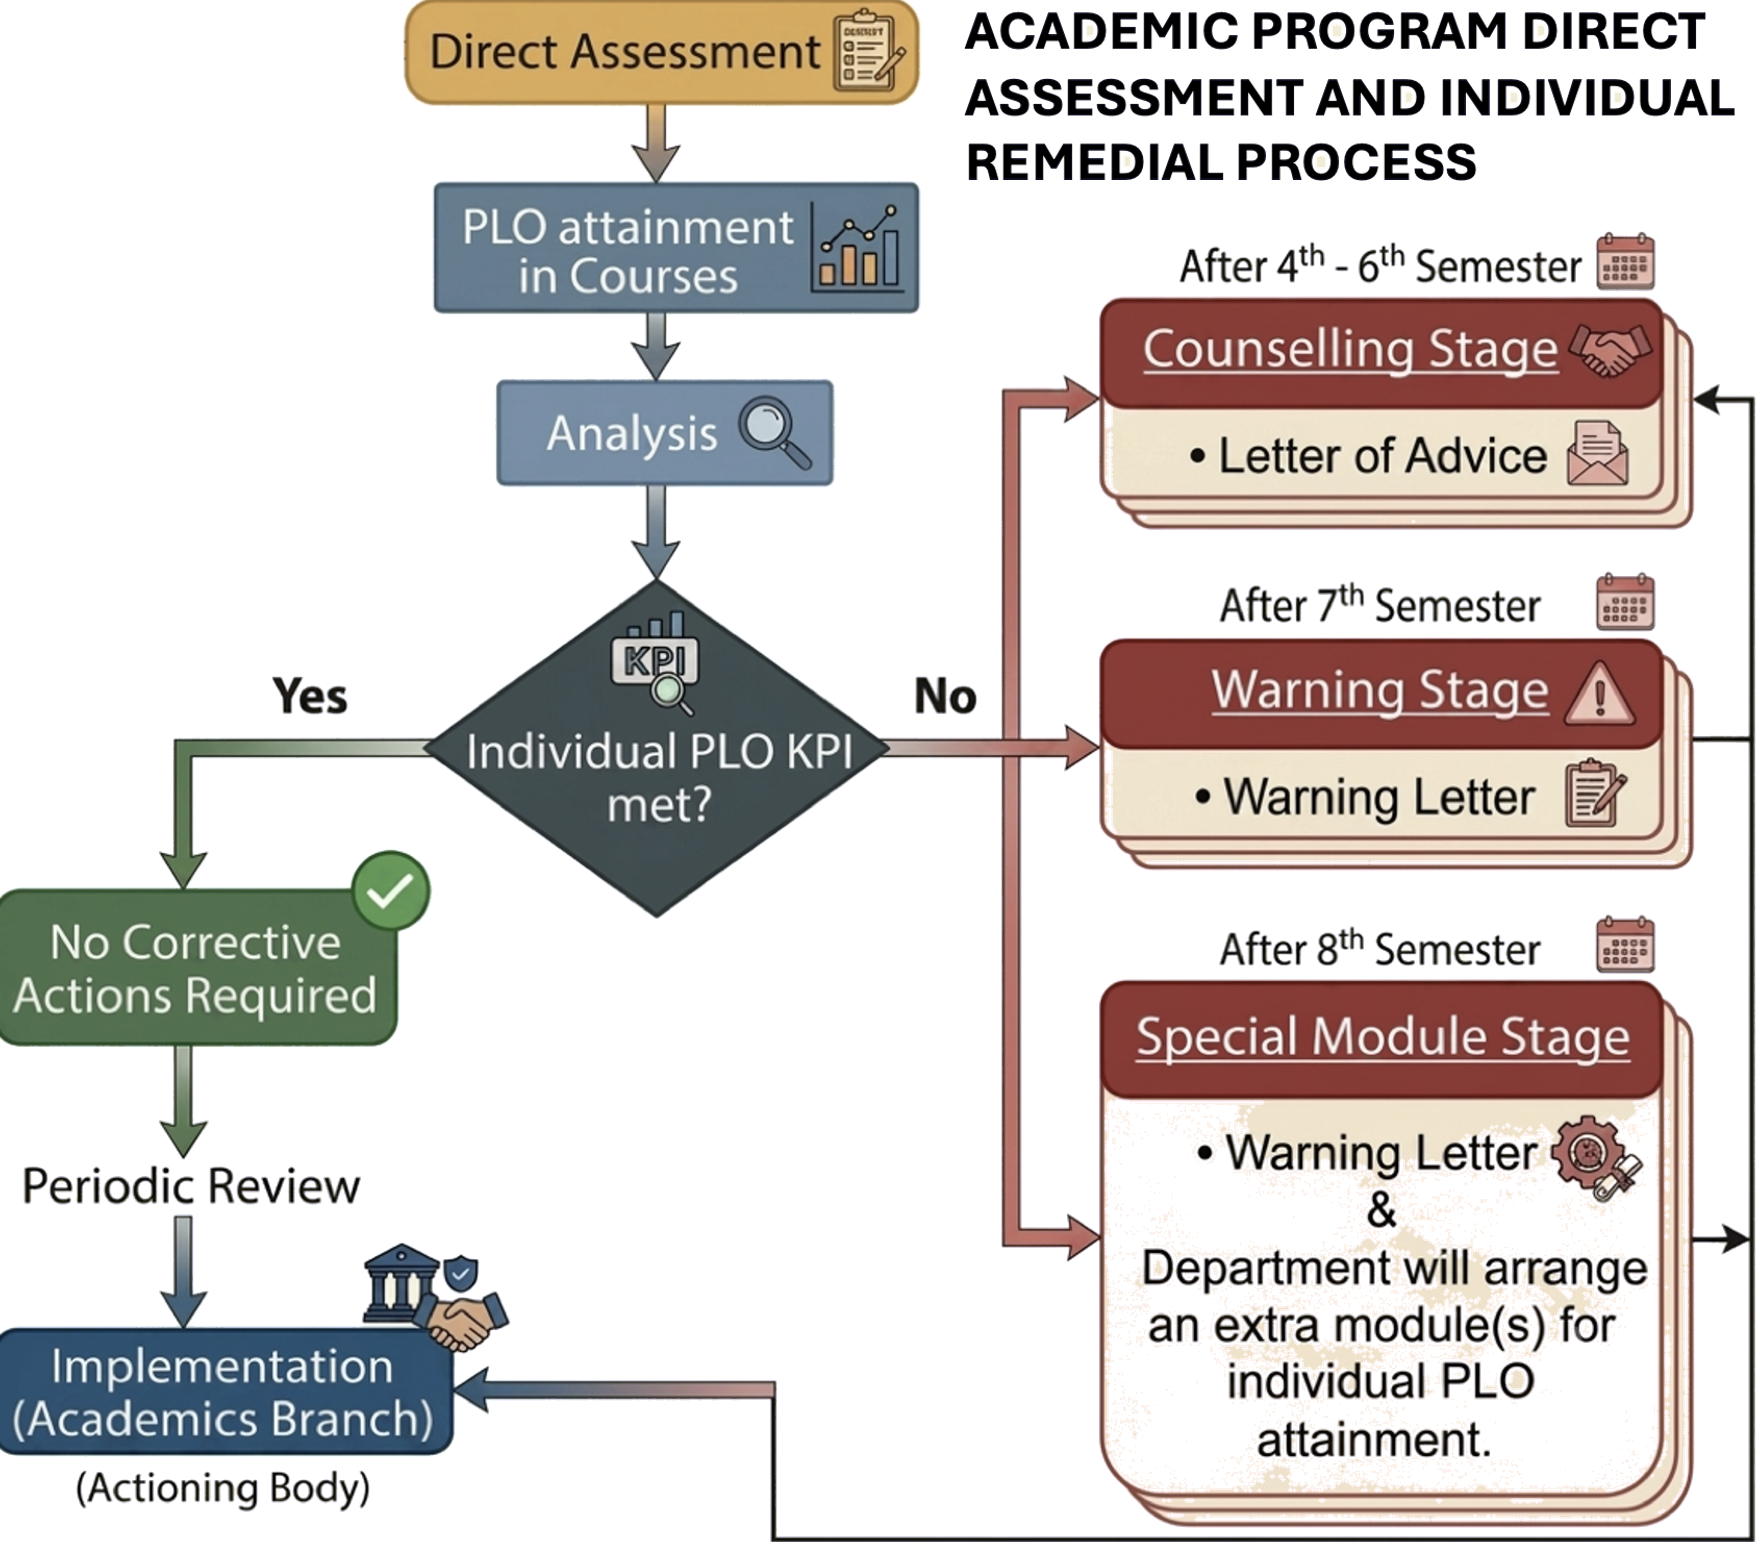
\includegraphics[width=0.7\textwidth]{images/front_matter/media/image-16.png}
\caption{Review of PLOs at Individual Level \& Corrective Actions}
\label{fig:individual level}
\end{figure}

\begin{enumerate}
\item \textbf{Counseling Stage (4\textsuperscript{th} -- 6\textsuperscript{th} Semester)}

At the end of each semester, the LQEC identifies students who have not met the required PLO attainment benchmark. Academic advisors or UG coordinators counsel these students and guide them on addressing the identified deficiencies through relevant courses and assessments in subsequent semesters. Where necessary, an advisory letter is issued to formally communicate the concern and recommended actions. A template counseling form is provided in Annexure~\ref{annex:counselling-form}.

\item \textbf{Warning Stage (7\textsuperscript{th} Semester)}

If a student continues to fall below the 50\% attainment benchmark for any PLO by the end of the 7\textsuperscript{th} semester, a formal warning letter is issued. The department reviews the deficient PLOs and, where the relevant outcome is not adequately addressed through coursework in the 8\textsuperscript{th} semester, arranges additional learning and assessment activities to help the student demonstrate the required attainment. A template warning letter is provided in Annexure~\ref{annex:warning-letter}. 

\item \textbf{Special Modules and Recovery of PLO Deficiencies}

Students who remain deficient in any PLO by the 8\textsuperscript{th} semester, or after completing their coursework, are required to undertake additional assessment activities designed to address the specific deficiency. These may include assignments, projects, case studies, or other relevant assessment tasks. Such activities may also be arranged during the summer semester, where required, to provide students with an opportunity to demonstrate the attainment of the deficient PLOs. The marks obtained through these additional assessments are used exclusively to determine PLO attainment and do not contribute to course grades.

\item \textbf{Degree Completion Requirement}

Students must meet the prescribed PLO attainment requirements to fulfil the program’s graduation requirements. A student who remains below the required attainment benchmark for any PLO must complete the prescribed recovery process and demonstrate the required attainment before the degree can be awarded. This process ensures that individual PLO deficiencies are identified systematically, communicated to students, and addressed through appropriate counseling, warnings, and additional assessment opportunities.
\end{enumerate}

%\hypertarget{sec:individual-plo}{%
%\paragraph{Individual Student PLO Achievement and Recovery of PLOs Deficiency}\label{sec:individual-plo}}

%The PLOs attainment is accomplished through direct and indirect assessments. Details of the PLOs to be assessed are provided in Section~\ref{sec:3.1plos}. For an individual student, the attainment of PLOs is required and in case of deficiency in PLOs attainment is ensured through passing of additional assignments.

%The LQEC under supervision of HoD Software Engineering, through the academic branch SEECS, is responsible for monitoring individual students' PLOs attainment. HoD Software Engineering to ensure individual students' PLOs deficiency recovery.

%Both direct and indirect assessment of PLOs for individuals usually takes place from 4\textsuperscript{th} semester at the end of each subsequent semester where the individual must achieve defined level of PLOs attainment as per KPI. At the end of each semester from the 4\textsuperscript{th} semester onwards, the LQEC of Software Engineering department will scrutinize individual PLO attainment along with semester results. Individual failing in PLOs attainment shall be informed through student academic advisors with information to HoD. Individual students will be counseled through respective student academic advisors to recover the failed PLOs that are repeated in the upcoming courses. In case of 8\textsuperscript{th} semester or a student who has completed all coursework and still PLO deficient, a letter of warning will be given to the student, and the department will arrange extra module(s) (in the form of assignment, project, case-study etc.) for individual PLO attainment. The marks attained in such CQI assessments will only be used for the attainment of related PLO of such a student. However, these marks will not be used for the calculation of the grade of the student in the related course in which the student has failed the PLO. The degree award requirements will not be considered fulfilled until the individual student has achieved the prescribed PLO KPI. These special assignments/exams will take place during the summer semester.
\subsection{Assessment-Driven Continuous Improvement of the Program}

The Software Engineering Program at SEECS uses the results of direct and indirect assessment of PLOs as a systematic input to the CQI process. Assessment results obtained through coursework, FYDP, internship feedback, and graduate exit surveys are reviewed by the LQEC to identify areas of unsatisfactory attainment, gaps in student achievement, and opportunities for further improvement. The findings are discussed within the relevant academic bodies, and corrective or improvement measures are initiated where required.

At the course level, CLO and PLO attainment results are reviewed at the end of each semester. Where deficiencies or comparatively lower attainment are identified, the results are used to review CLO formulation, Bloom's Taxonomy levels, CLO-to-PLO mapping, course contents, teaching and learning strategies, and assessment methods. The CQI process therefore provides a mechanism for progressively improving course delivery and ensuring that assessments appropriately measure the intended learning outcomes. Course outlines are reviewed and revised where necessary, with changes made through the established academic approval process.

At the program level, cohort-level PLO attainment is analyzed to determine whether the prescribed KPIs are being achieved. The results from coursework and FYDP are considered together with indirect evidence obtained from employers through internship feedback and from graduating students through the Graduate Exit Survey. This triangulation of direct and indirect evidence enables the program to identify areas requiring further attention from both academic and professional perspectives. For example, areas showing comparatively lower attainment in problem analysis, design and development, sustainability, professional skills, or familiarity with modern tools can provide input for strengthening curriculum content, practical and design-oriented activities, professional skills development, and industry exposure.

The internship feedback provides an industry perspective on the competencies demonstrated by students in professional environments. The feedback is used to identify areas where workplace competencies can be further strengthened, particularly in complex problem-solving, system design, sustainability, teamwork, and professional conduct. Similarly, the Graduate Exit Survey provides students' perceptions of their attainment of PLOs and highlights areas that may require additional attention in curriculum content, practical exposure, assessment strategies, and professional development activities.

The assessment results are also used to monitor individual student attainment. Students who do not achieve the prescribed PLO KPI are identified through the periodic review of individual PLO attainment. Such students are counseled through their academic advisors and provided opportunities to recover deficient PLOs through subsequent coursework. Where a student remains deficient after completion of coursework, additional assignments, projects, case studies, or other assessment modules are arranged to ensure attainment of the deficient PLOs before fulfillment of degree award requirements.

The overall process establishes a closed-loop mechanism in which assessment results are collected, analyzed, reviewed, and translated into improvement actions. The effectiveness of these actions is subsequently monitored through further assessment cycles. Thus, the program's PLO attainment data, stakeholder feedback, and CQI reviews provide continuous input for the progressive improvement of curriculum mapping, course design, teaching and learning practices, assessment mechanisms, practical and design experiences, and professional development opportunities. In this manner, assessment is not limited to measuring student achievement but serves as an integral mechanism for the continued development and improvement of the BE Software Engineering Program.
%-----------------------------------------------------------------------
\hypertarget{sec:materials}{%
\section{Materials used in Demonstration for Attainment of PLOs}\label{sec:materials}}

The Software Engineering Program uses a comprehensive set of academic and assessment materials to demonstrate the achievement of PLOs. These include approved course outlines containing CLOs, PLO mappings, Bloom's Taxonomy levels, course contents, and assessment methods. CLO and PLO attainment reports generated through the Qalam OBE system and course assessment evidence such as examinations, quizzes, assignments, laboratory work, projects, presentations, and assessment rubrics are employed for this purpose.

For the Final Year Design Project (FYDP), evidence includes proposal and mid-semester defense assessments, SRS and SDS documents, project progress evaluations, final reports, final defense, oral presentations, and corresponding assessment rubrics. Individual and cohort-level PLO attainment records are also maintained to demonstrate achievement against the prescribed KPIs.

In addition to direct assessment evidence, indirect assessment materials include employer internship feedback forms and analyses, as well as Graduate Exit Survey forms and analyses. These materials collectively provide direct and indirect evidence of PLO achievement and support the review of attainment through the CQI process. The consolidated evidence is maintained through Qalam, academic records, SEECS assessment systems, and relevant SAR annexures.

